\chapter{Sistema multisensorial }
\label{cap:capitulo4}

%\begin{flushright}
%\begin{minipage}[]{10cm}
%\emph{Quizás algún fragmento de libro inspirador...}\\
%\end{minipage}\\

%Autor, \textit{Título}\\
%\end{flushright}

\vspace{1cm}
Este capítulo consta de la descripción detallada del proceso que se ha llevado a cabo para crear el sistema multisensorial para la monitorización de animales de laboratorio. 

La base idea de este trabajo ha sido pensada para un laboratorio de animales, ya que la robótica está presente en este ámbito, así como en otros muchos, a pesar de que en este sector no trabajan ingenieros. Debido a este motivo, puede haber trabajo que se realice en el laboratorio que podría mejorarse hasta incluso automatizarse. 

Para obtener más información, se ha contactado con el laboratorio de animales de la Universidad de Alcalá de Henares \footnote{\url{https://www.uah.es/es/}}  para conocer la situación en la que trabajan. Se han apreciado bastantes cosas mejorables y se ha enfocado el objetivo en el estudio de los ratones del laboratorio, que requieren una observación constante así como del entorno en el que se encuentran debido a que deben estar bajo unas condiciones determinadas.\\

Después de conocer esta información la idea del trabajo ha tomado más forma e idea, decidiendo así componer un sistema multisensorial. Este sistema consiste en dotar a un computador de diferentes sensores que le permitan obtener datos del entorno que le rodea para poder actuar en función a ellos. 

Asimismo, debido al desconocimiento de los trabajadores del laboratorio del mundo de la robótica y la ingeniería en general, se ofrece una interfaz gráfica donde los valores numéricos obtenidos por los sensores, así como cualquier interacción necesaria se traducen en \textit{widgets} comprensibles para cualquier usuario de una manera intuitiva y sencilla.\\

Dos son las partes esenciales para el desarrollo: hardware y software. En la primera sección se presenta el desarrollo hardware y en la sección posterior el desarrollo software que se ha realizado sobre la configuración hardware.


\section{Hardware}
La placa que se ha utilizado para el proyecto es la Raspberry Pi 4B (Figura \ref{fig:rasp}), el último modelo de Raspberry y muy utilizada para el desarrollo de proyectos debido a su bajo coste. Este modelo es el más rápido y potente, ofreciendo de dos a tres veces el rendimiento del procesador de su modelo predecesor. El sistema operativo que utiliza la Raspberry es Raspbian.
\begin{figure} [h!]
  \begin{center}
    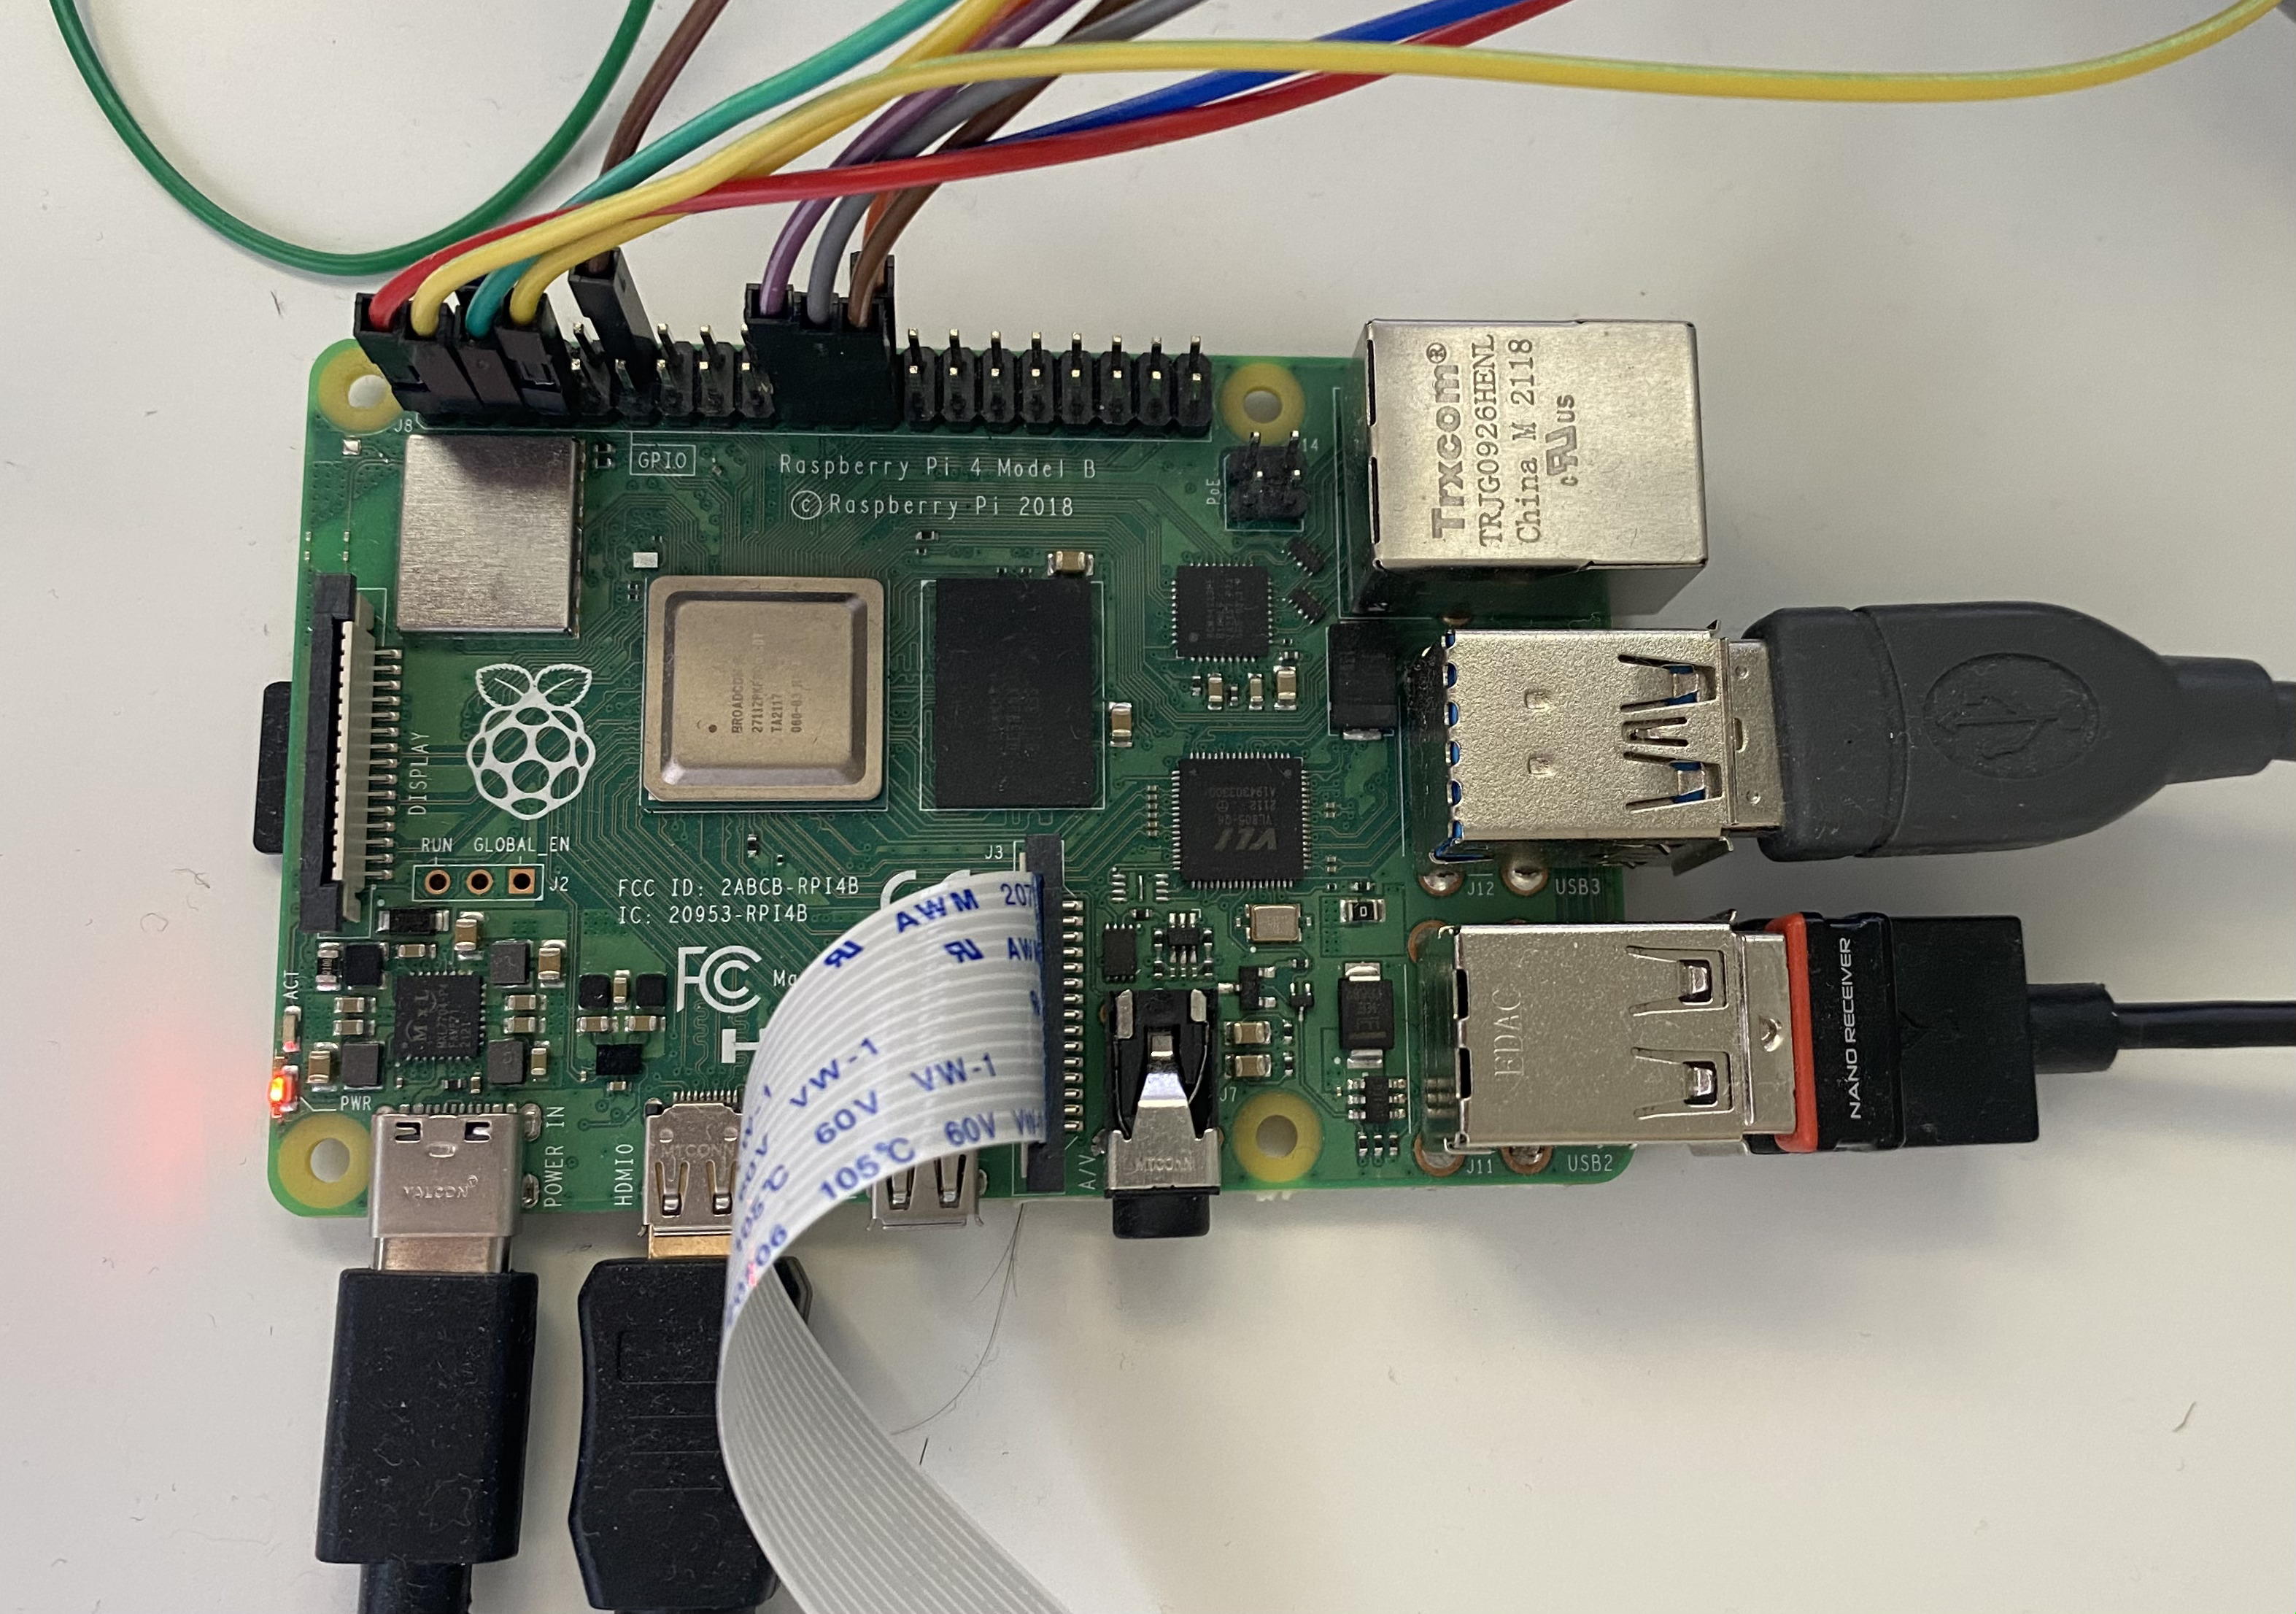
\includegraphics[width=8cm]{figs/raspberry}
  \end{center}
  \caption{Raspberry Pi 4B}
  \label{fig:rasp}
\end{figure}\\

Está dotada de una serie de pines y puertos que permiten su conexión con distintos sensores o actuadores. Para este trabajo se han utilizado los siguientes sensores:
\begin{itemize}
\item{Sensor BME680 (Figura \ref{fig:bme}).} Este sensor es capaz de medir hasta cuatro parámetros: el gas, la temperatura, la presión y la humedad.
\begin{figure} [h!]
  \begin{center}
    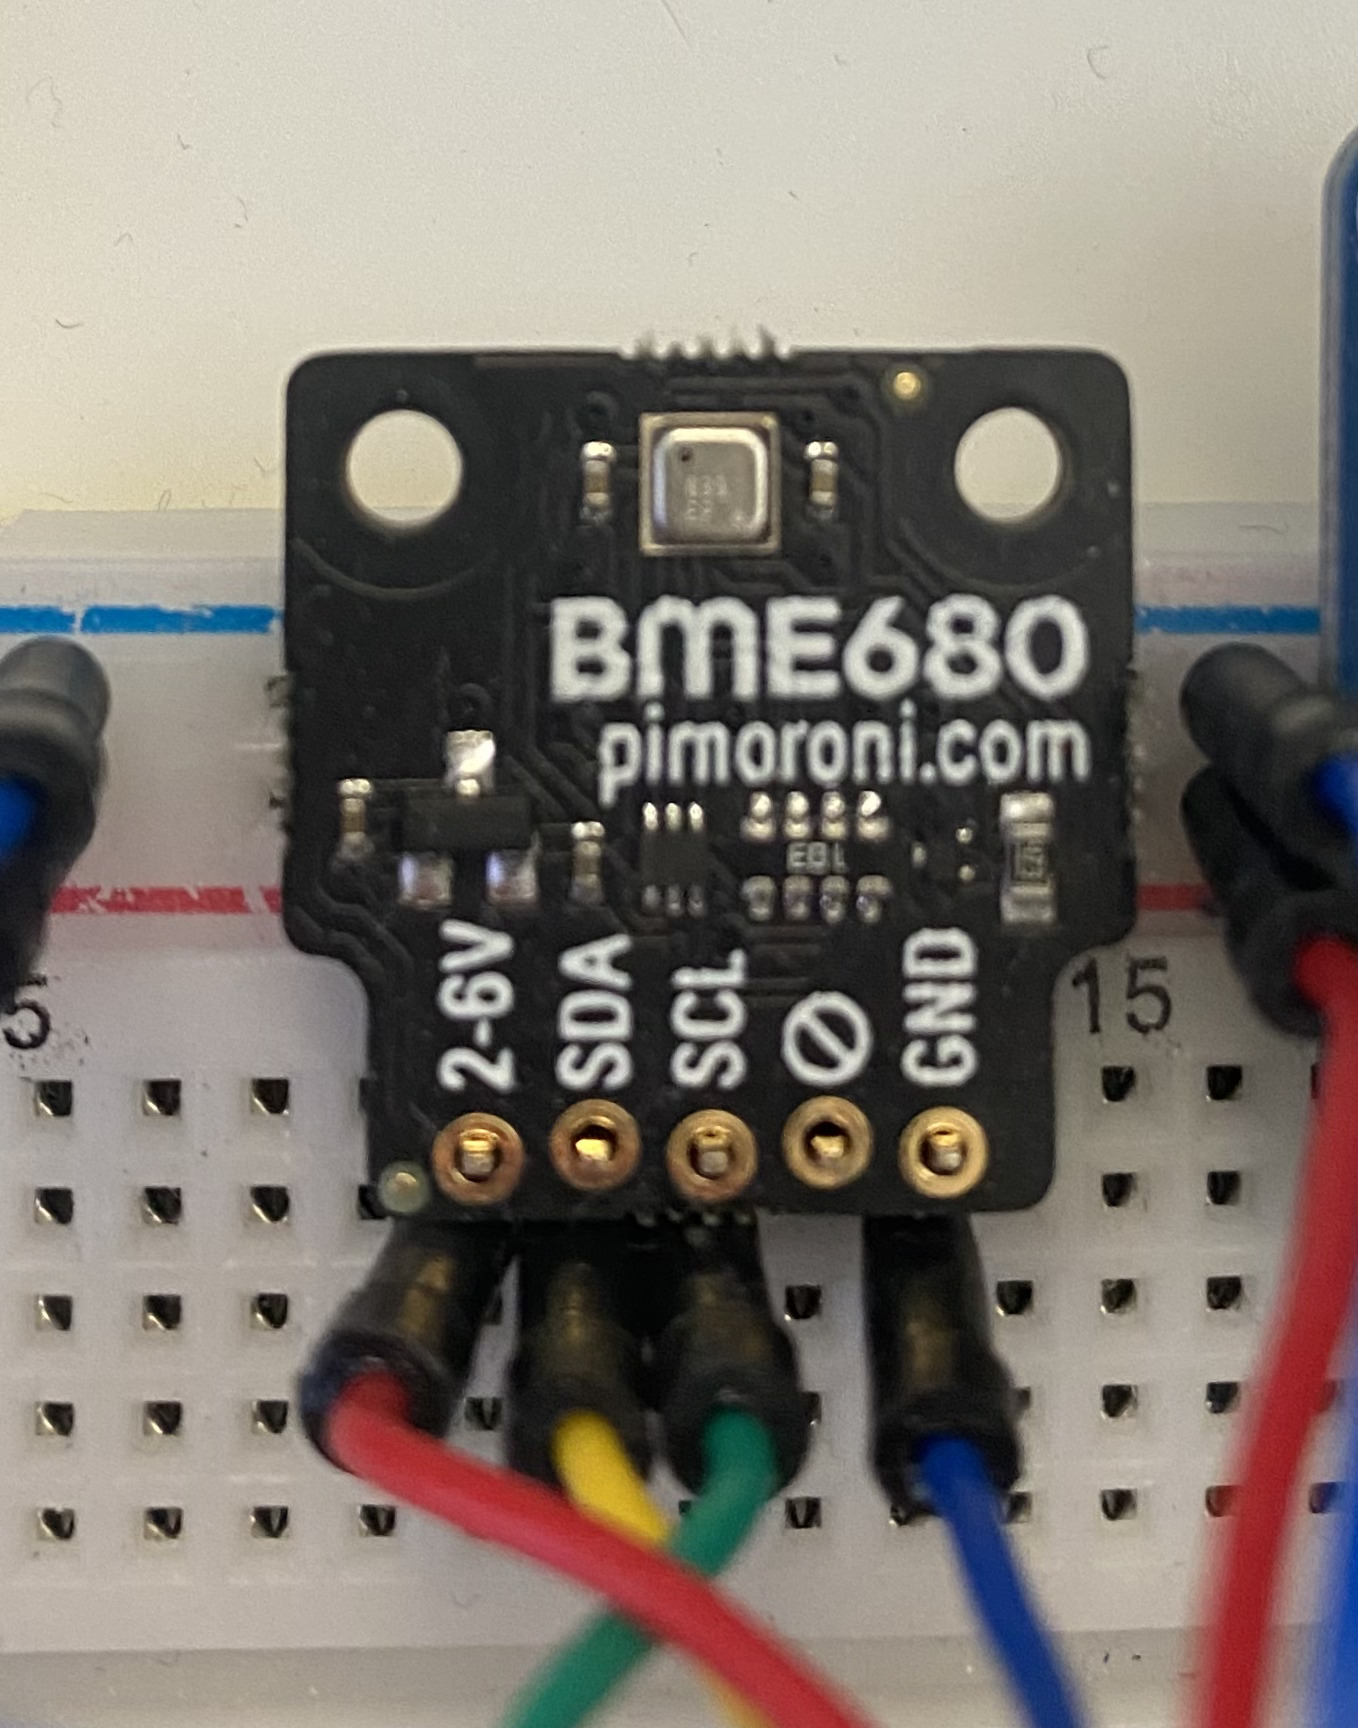
\includegraphics[width=6cm]{figs/bme}
  \end{center}
  \caption{Sensor BME680.}
  \label{fig:bme}
\end{figure}\\

\item{Sensor AMG8833 (Figura \ref{fig:amg}).} Este sensor es una cámara térmica que permite recibir la información del entorno y mostrarla a través de un rango de colores. Los colores más cálidos ---como el rojo--- indican la presencia de mayor temperatura, mientras que los colores fríos ---como el azul--- indican una temperatura inferior. Los valores que ofrece este sensor son una lista de 8x8 valores, que debe ser traducida para mostrar una imagen.
\begin{figure} [h!]
  \begin{center}
    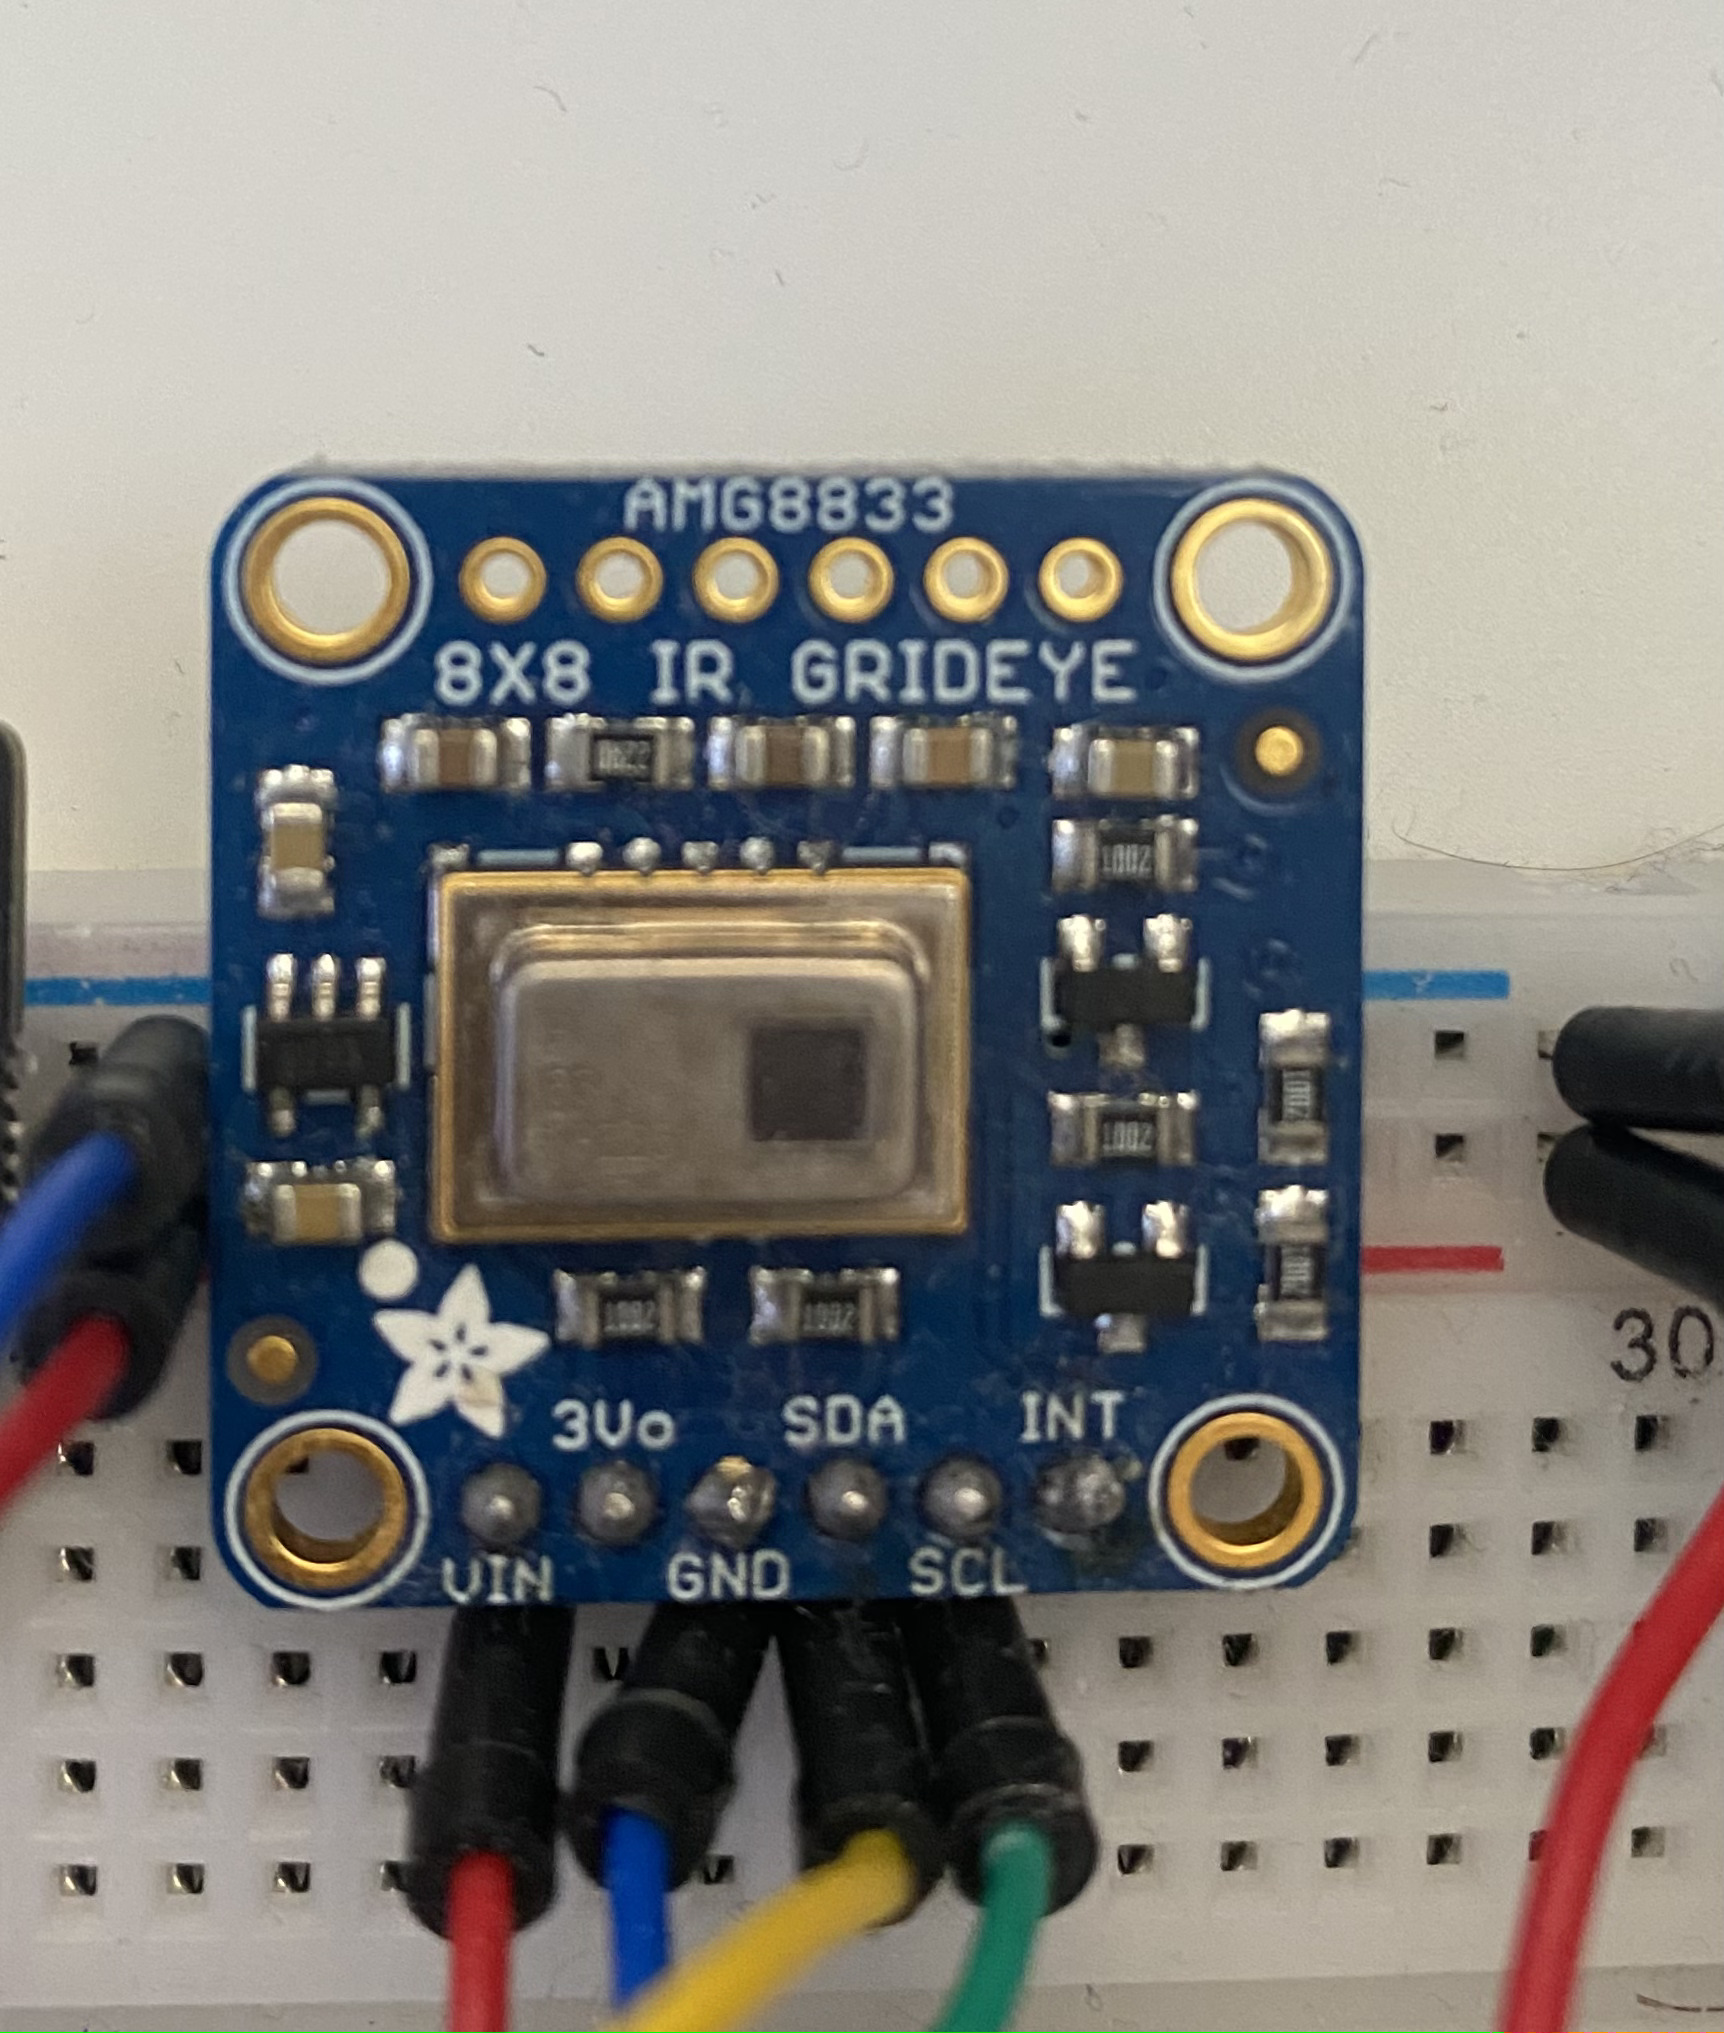
\includegraphics[width=6cm]{figs/amg}
  \end{center}
  \caption{Sensor AMG8833.}
  \label{fig:amg}
\end{figure}\\

\item{Sensor DS18B20 (Figura \ref{fig:ds}).} Este sensor permite medir la temperatura en superficies húmedas, ya que es resistente al agua.
\begin{figure} [h!]
  \begin{center}
    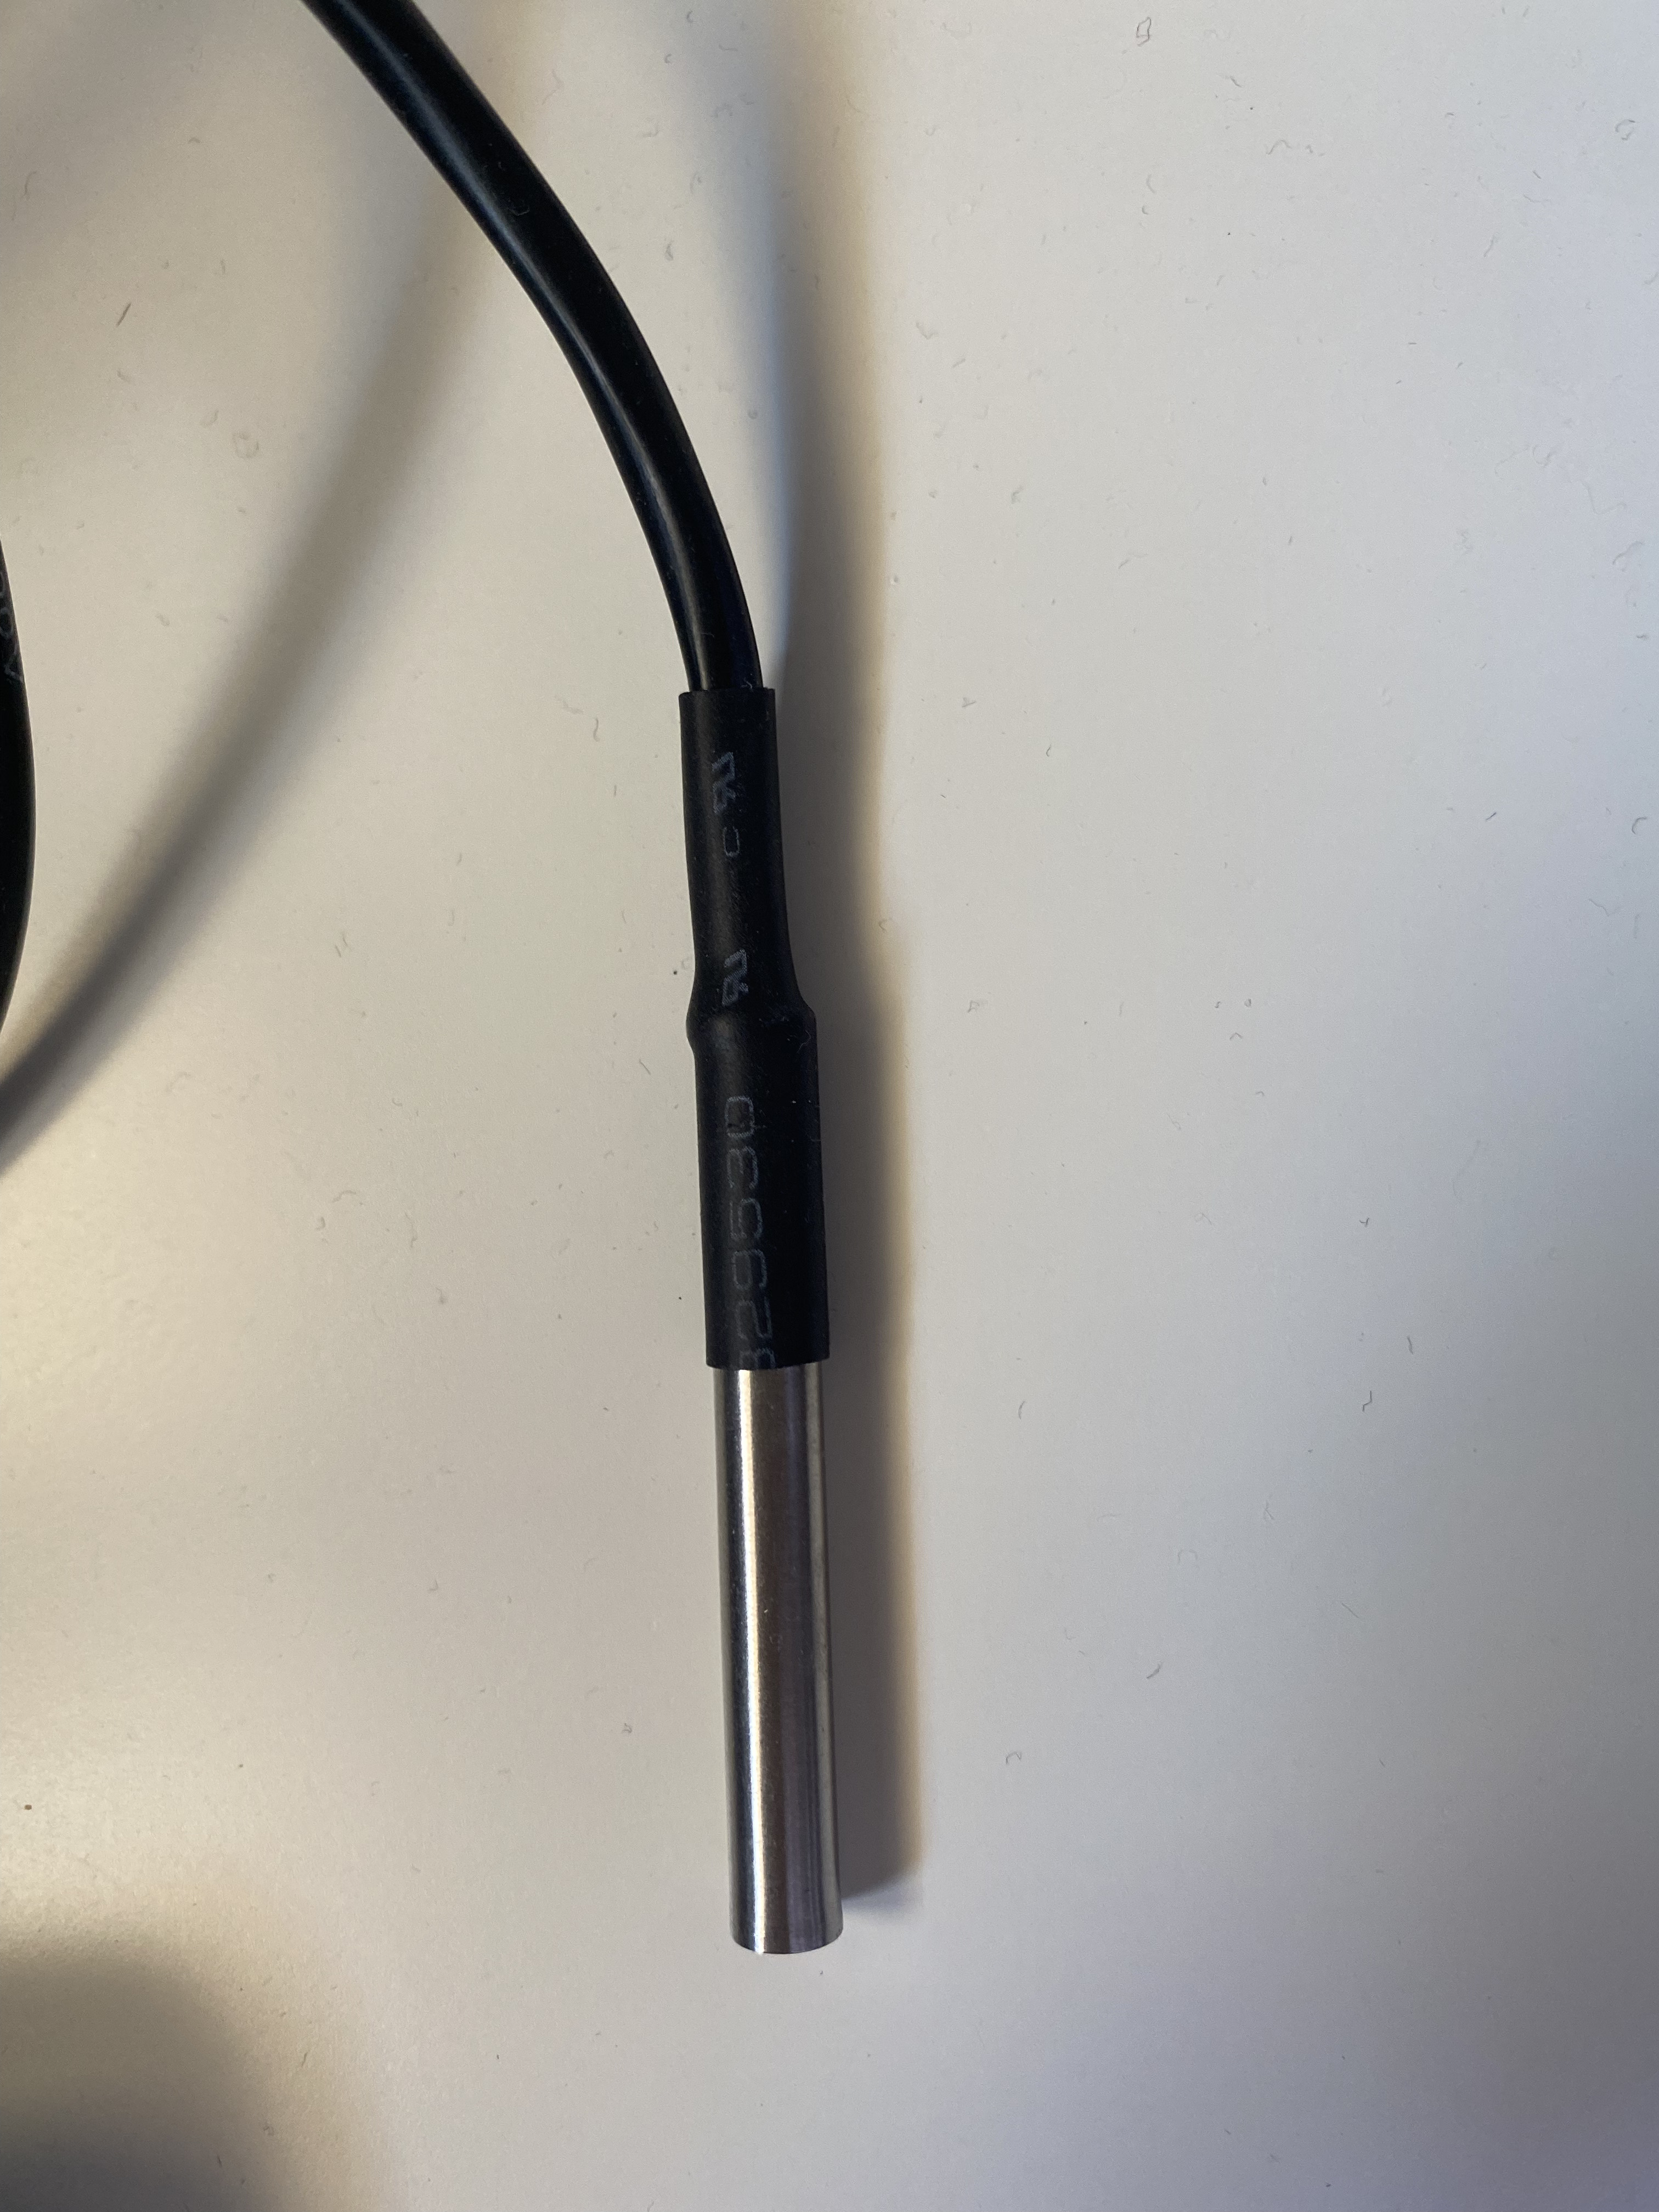
\includegraphics[width=6cm]{figs/ds}
  \end{center}
  \caption{Sensor DS18B20.}
  \label{fig:ds}
\end{figure}\\

\item{MQ-135 (Figura \ref{fig:mq}).} Este sensor permite medir la calidad de distintos gases, entre ellos el de amoníaco. Este sensor tiene lecturas analógicas, por lo que es necesario el uso de un conversor analógico a digital.
\begin{figure} [h!]
  \begin{center}
    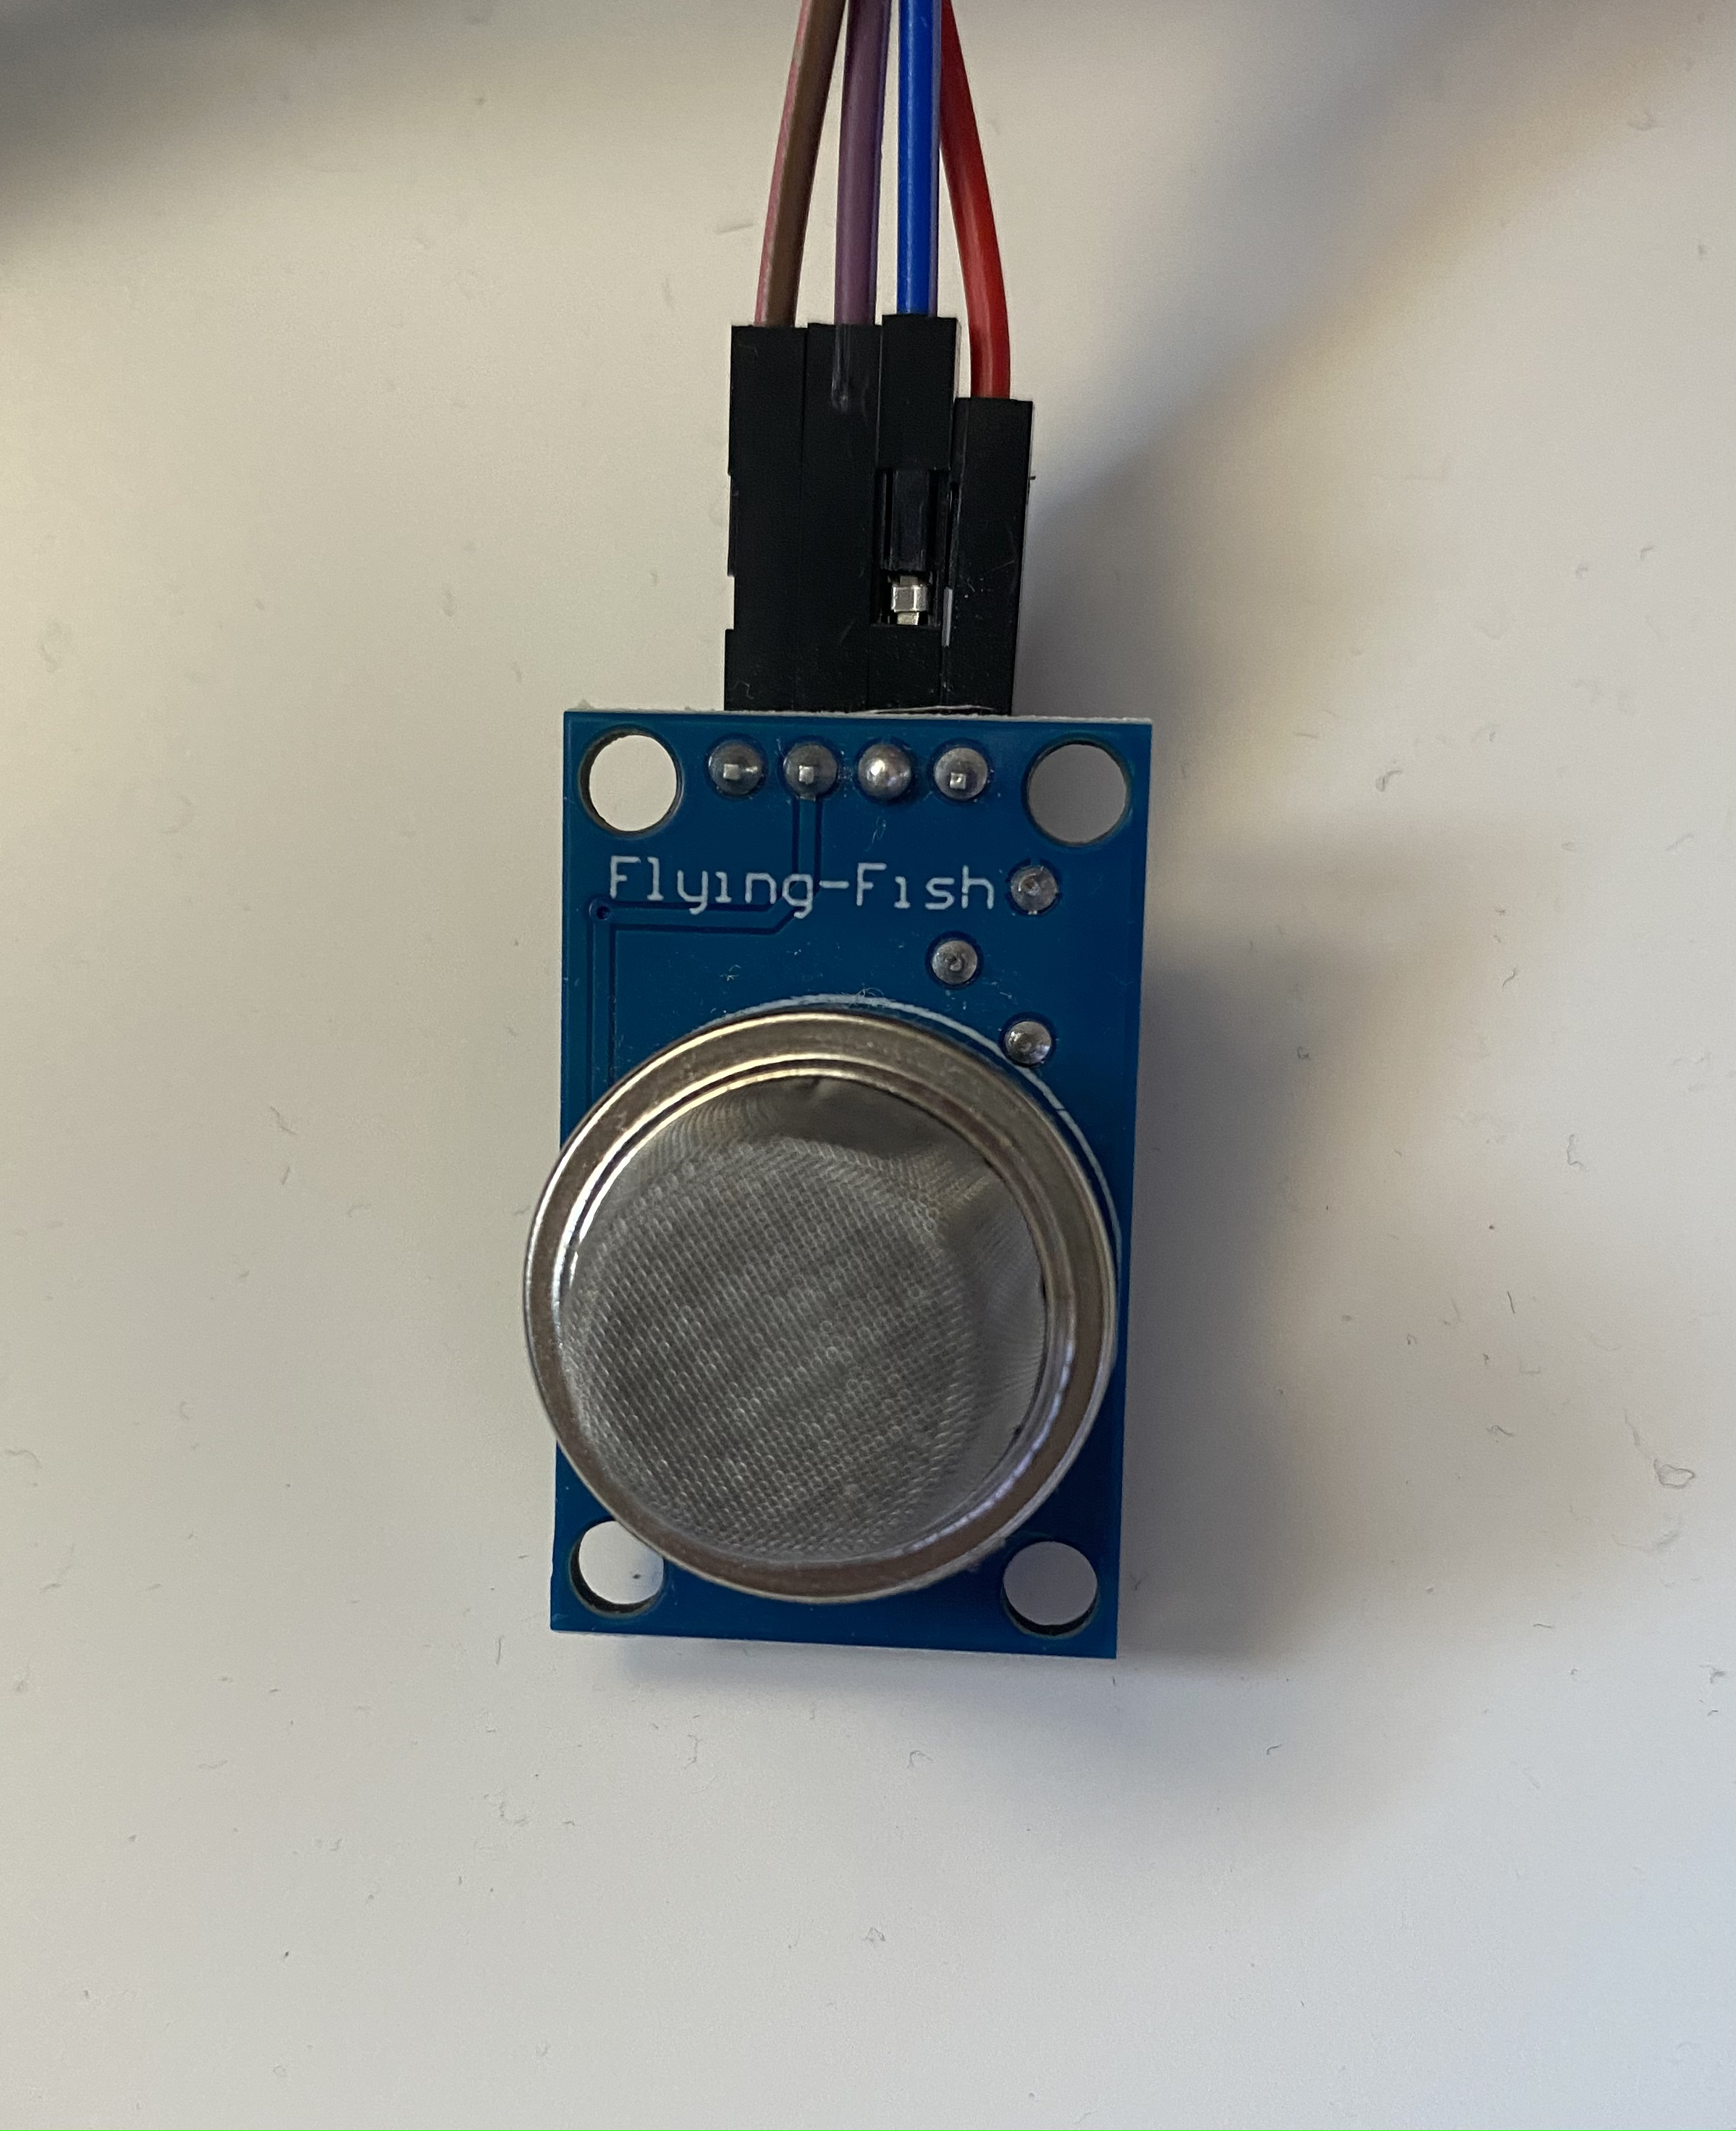
\includegraphics[width=6cm]{figs/mq}
  \end{center}
  \caption{Sensor MQ-135.}
  \label{fig:mq}
\end{figure}\\

\item{Sensor nivel de agua (Figura \ref{fig:nivel}).} Con este sensor se puede medir la presencia de agua, así como la cantidad de agua que hay. Este sensor tiene lecturas analógicas, por lo que es necesario el uso de un conversor analógico a digital.
\begin{figure} [h!]
  \begin{center}
    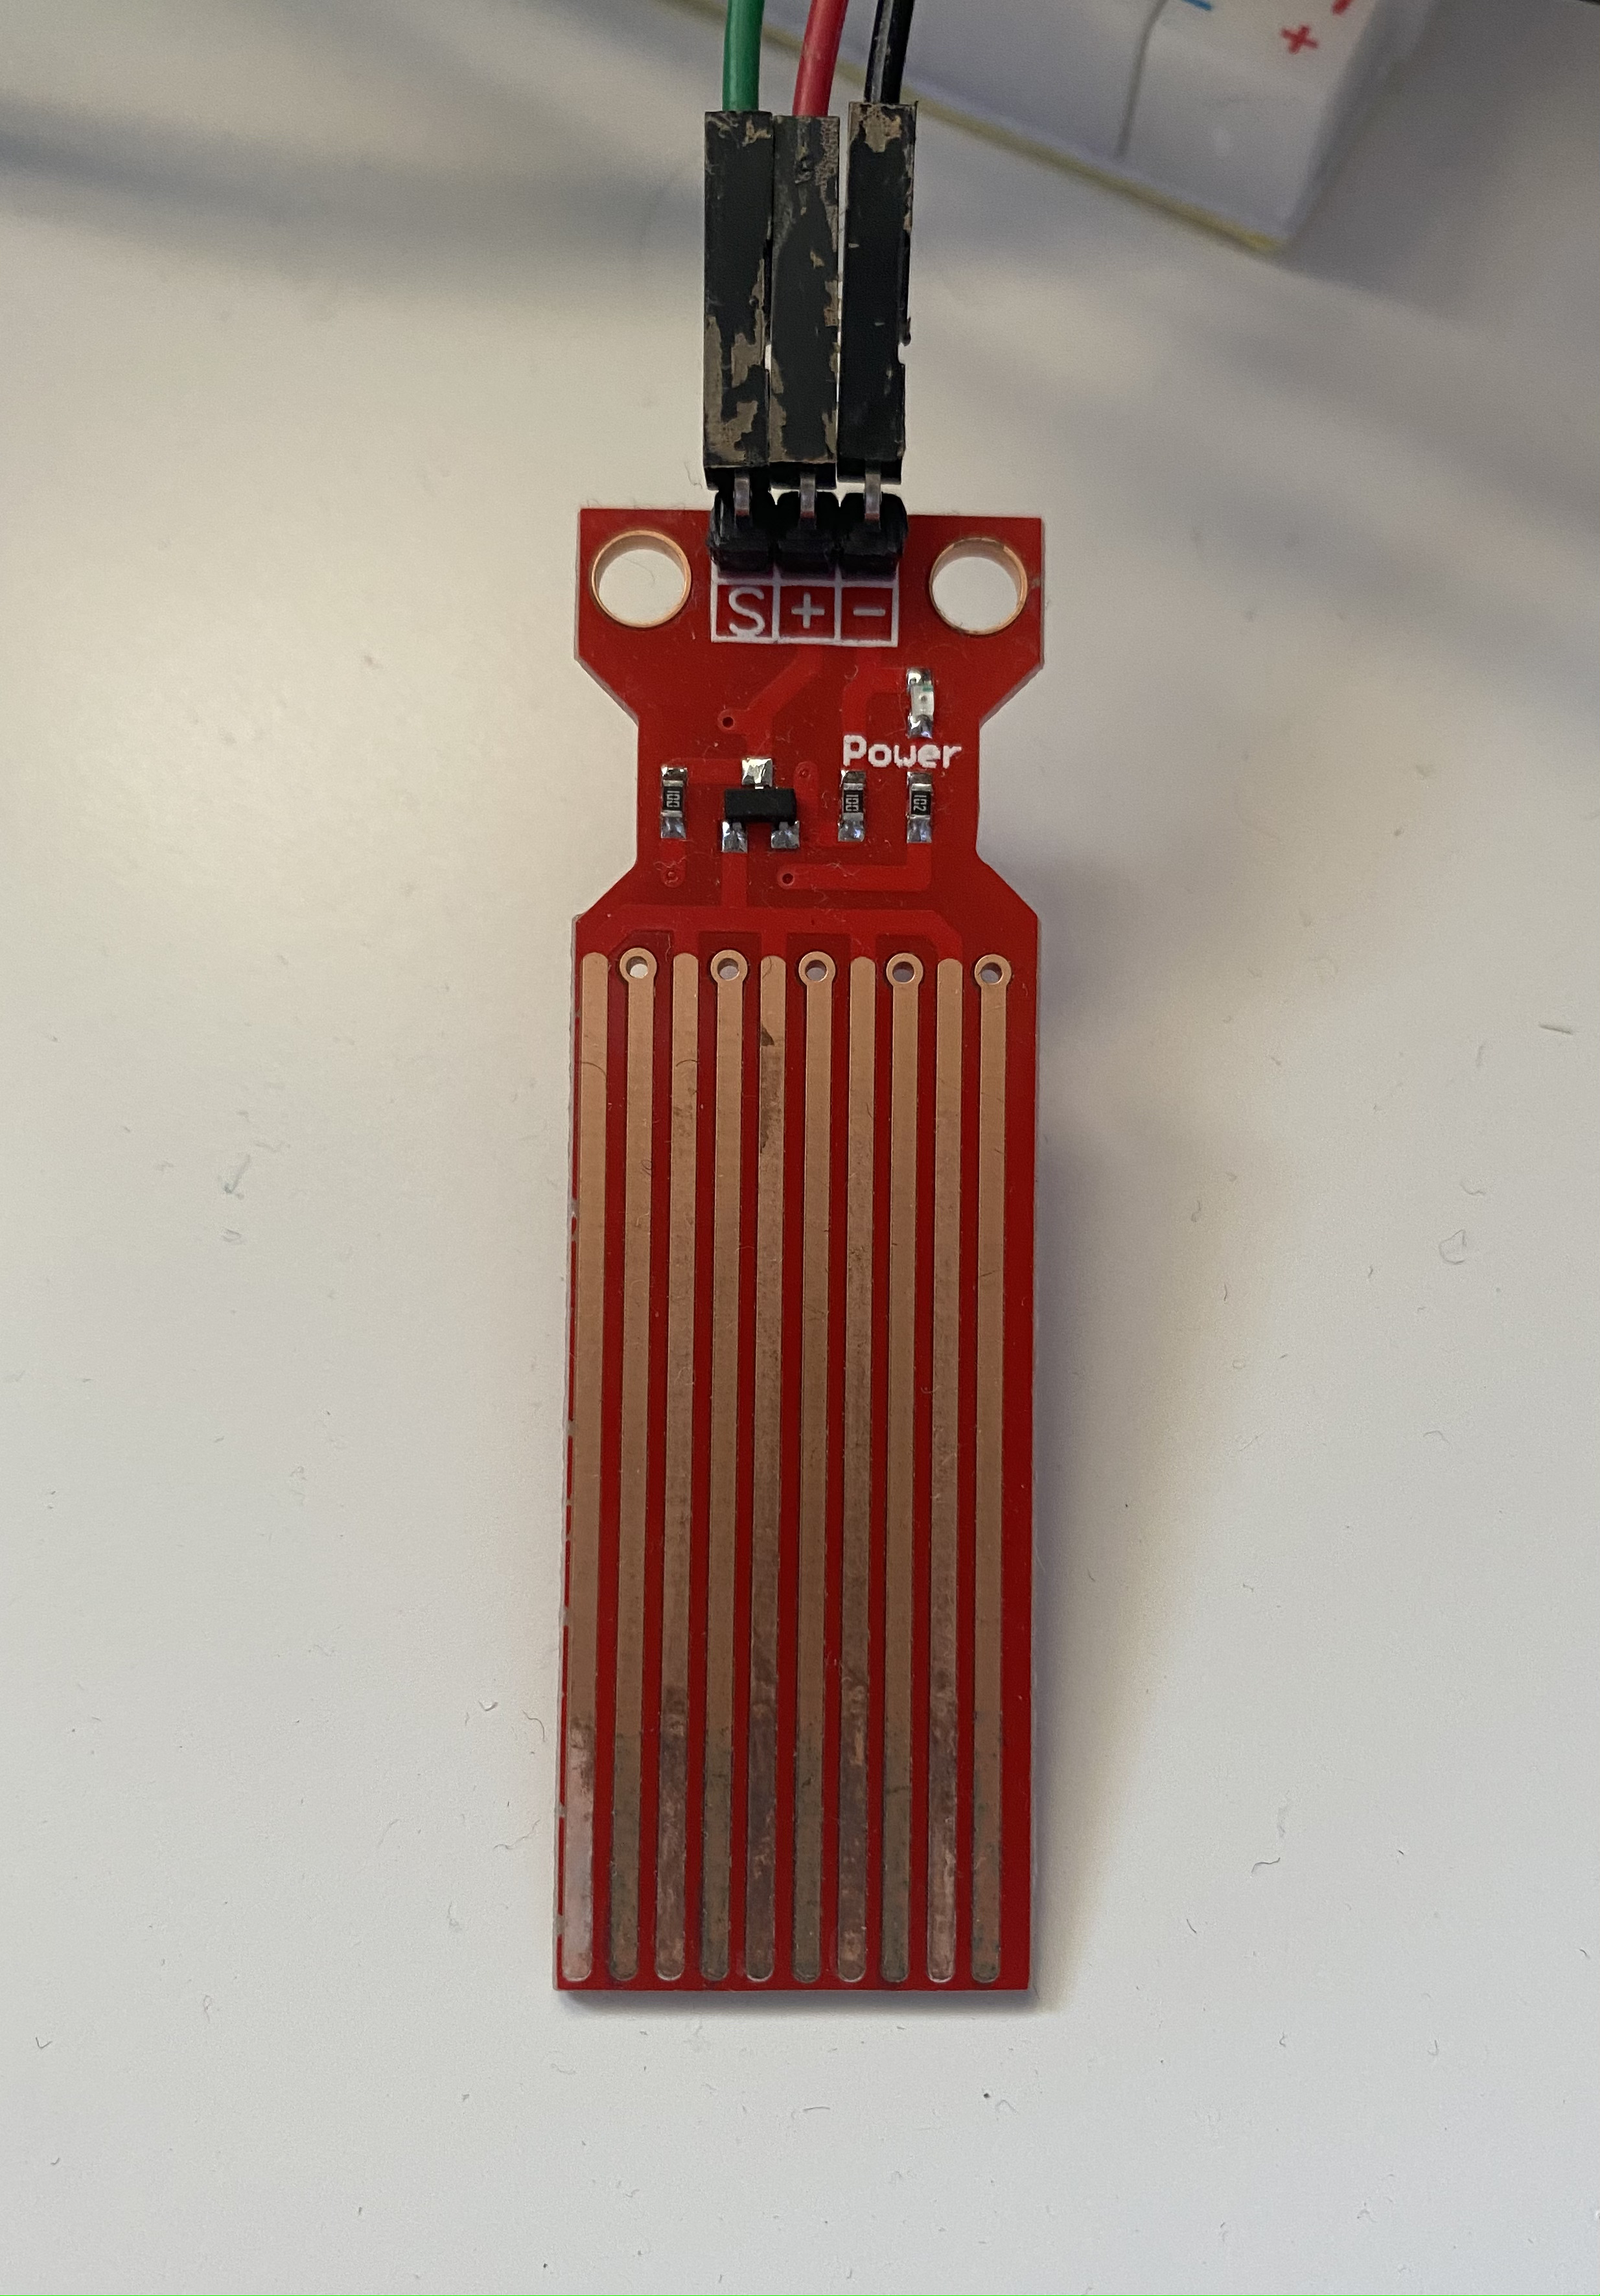
\includegraphics[width=6cm]{figs/nivel}
  \end{center}
  \caption{Sensor de nivel de agua.}
  \label{fig:nivel}
\end{figure}\\

%\item{Sensor AM2315 (Figura \ref{fig:am}).} Este sensor permite medir tanto la temperatura como la humedad.
%\begin{figure} [h!]
%  \begin{center}
%    \includegraphics[width=6cm]{figs/am}
%  \end{center}
%  \caption{Sensor AM2315.}
%  \label{fig:ds}
%\end{figure}\\

\item{Seek thermal (Figura \ref{fig:seek}).} Este sensor es una cámara térmica. Permite obtener imágenes representando las temperaturas con colores de la misma forma que el sensor \ref{fig:amg}, pero con mucha más calidad y precisión.\begin{figure} [h!]
  \begin{center}
    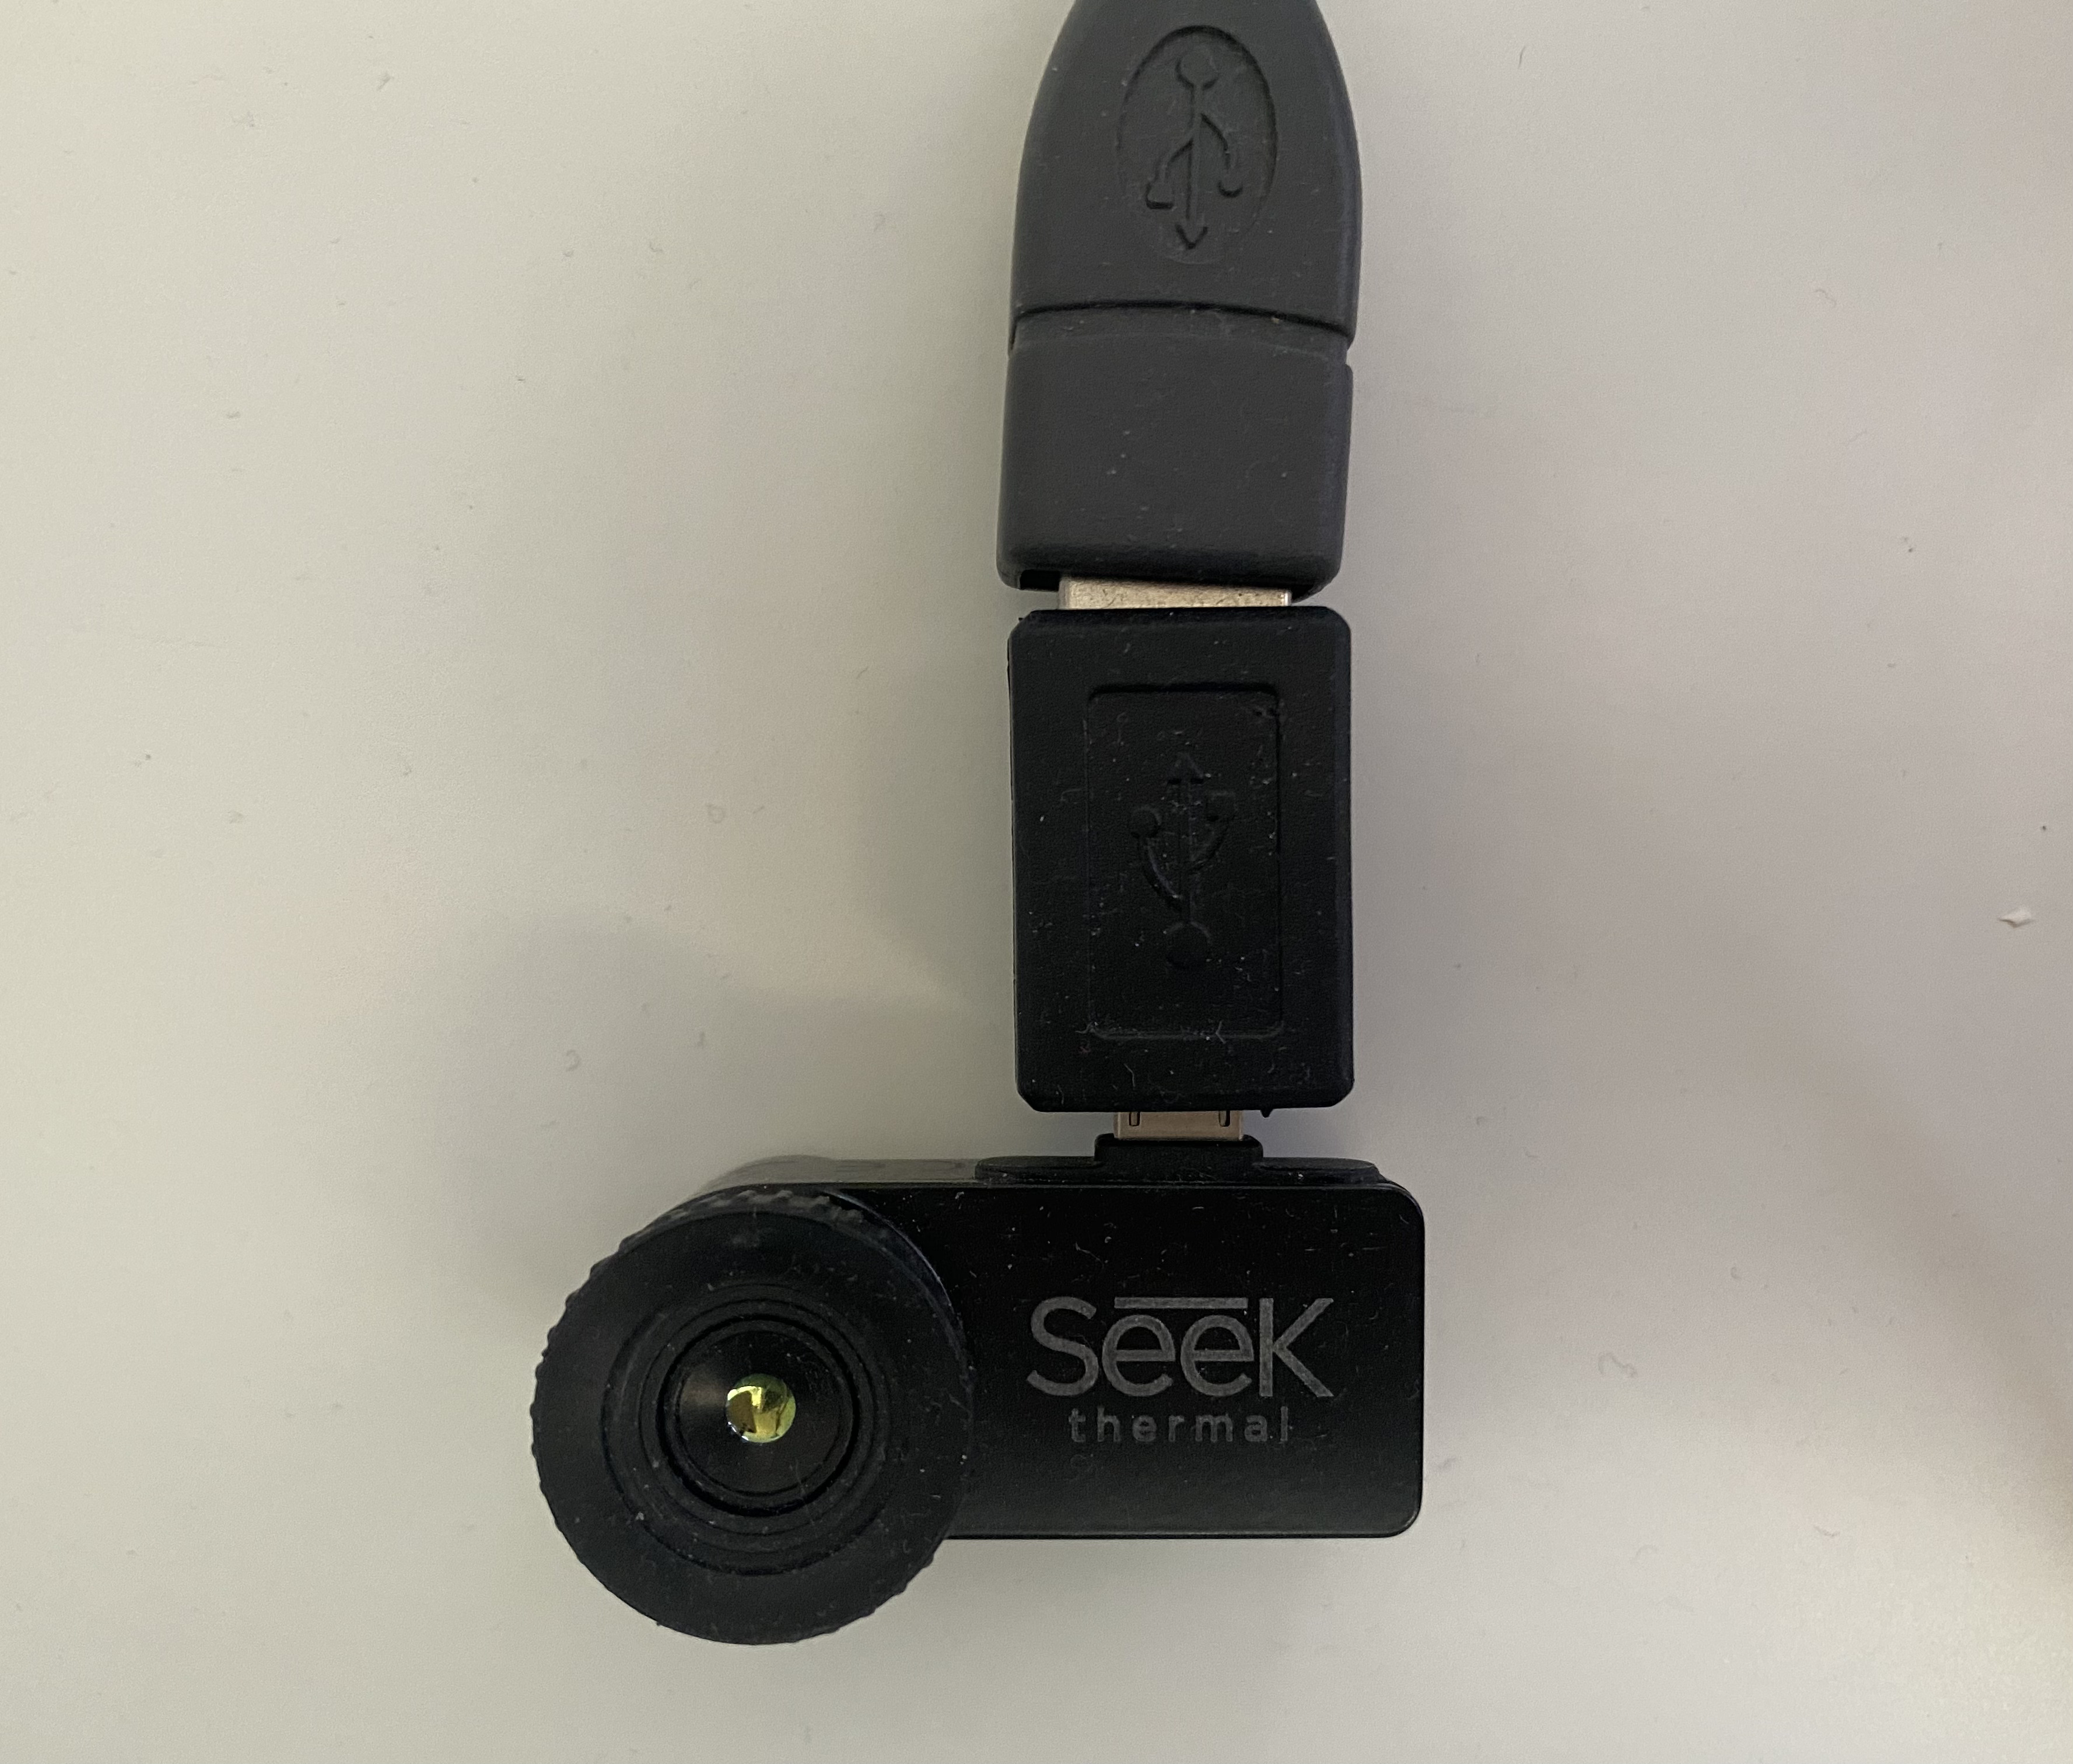
\includegraphics[width=6cm]{figs/seek}
  \end{center}
  \caption{Cámara térmica.}
  \label{fig:seek}
\end{figure}\\

\item{PiCamera (Figura \ref{fig:picam}).} Este sensor es una de las cámaras oficiales de Raspberry, que permite obtener imágenes del entorno y mostrarlas en pantalla.
\begin{figure} [h!]
  \begin{center}
    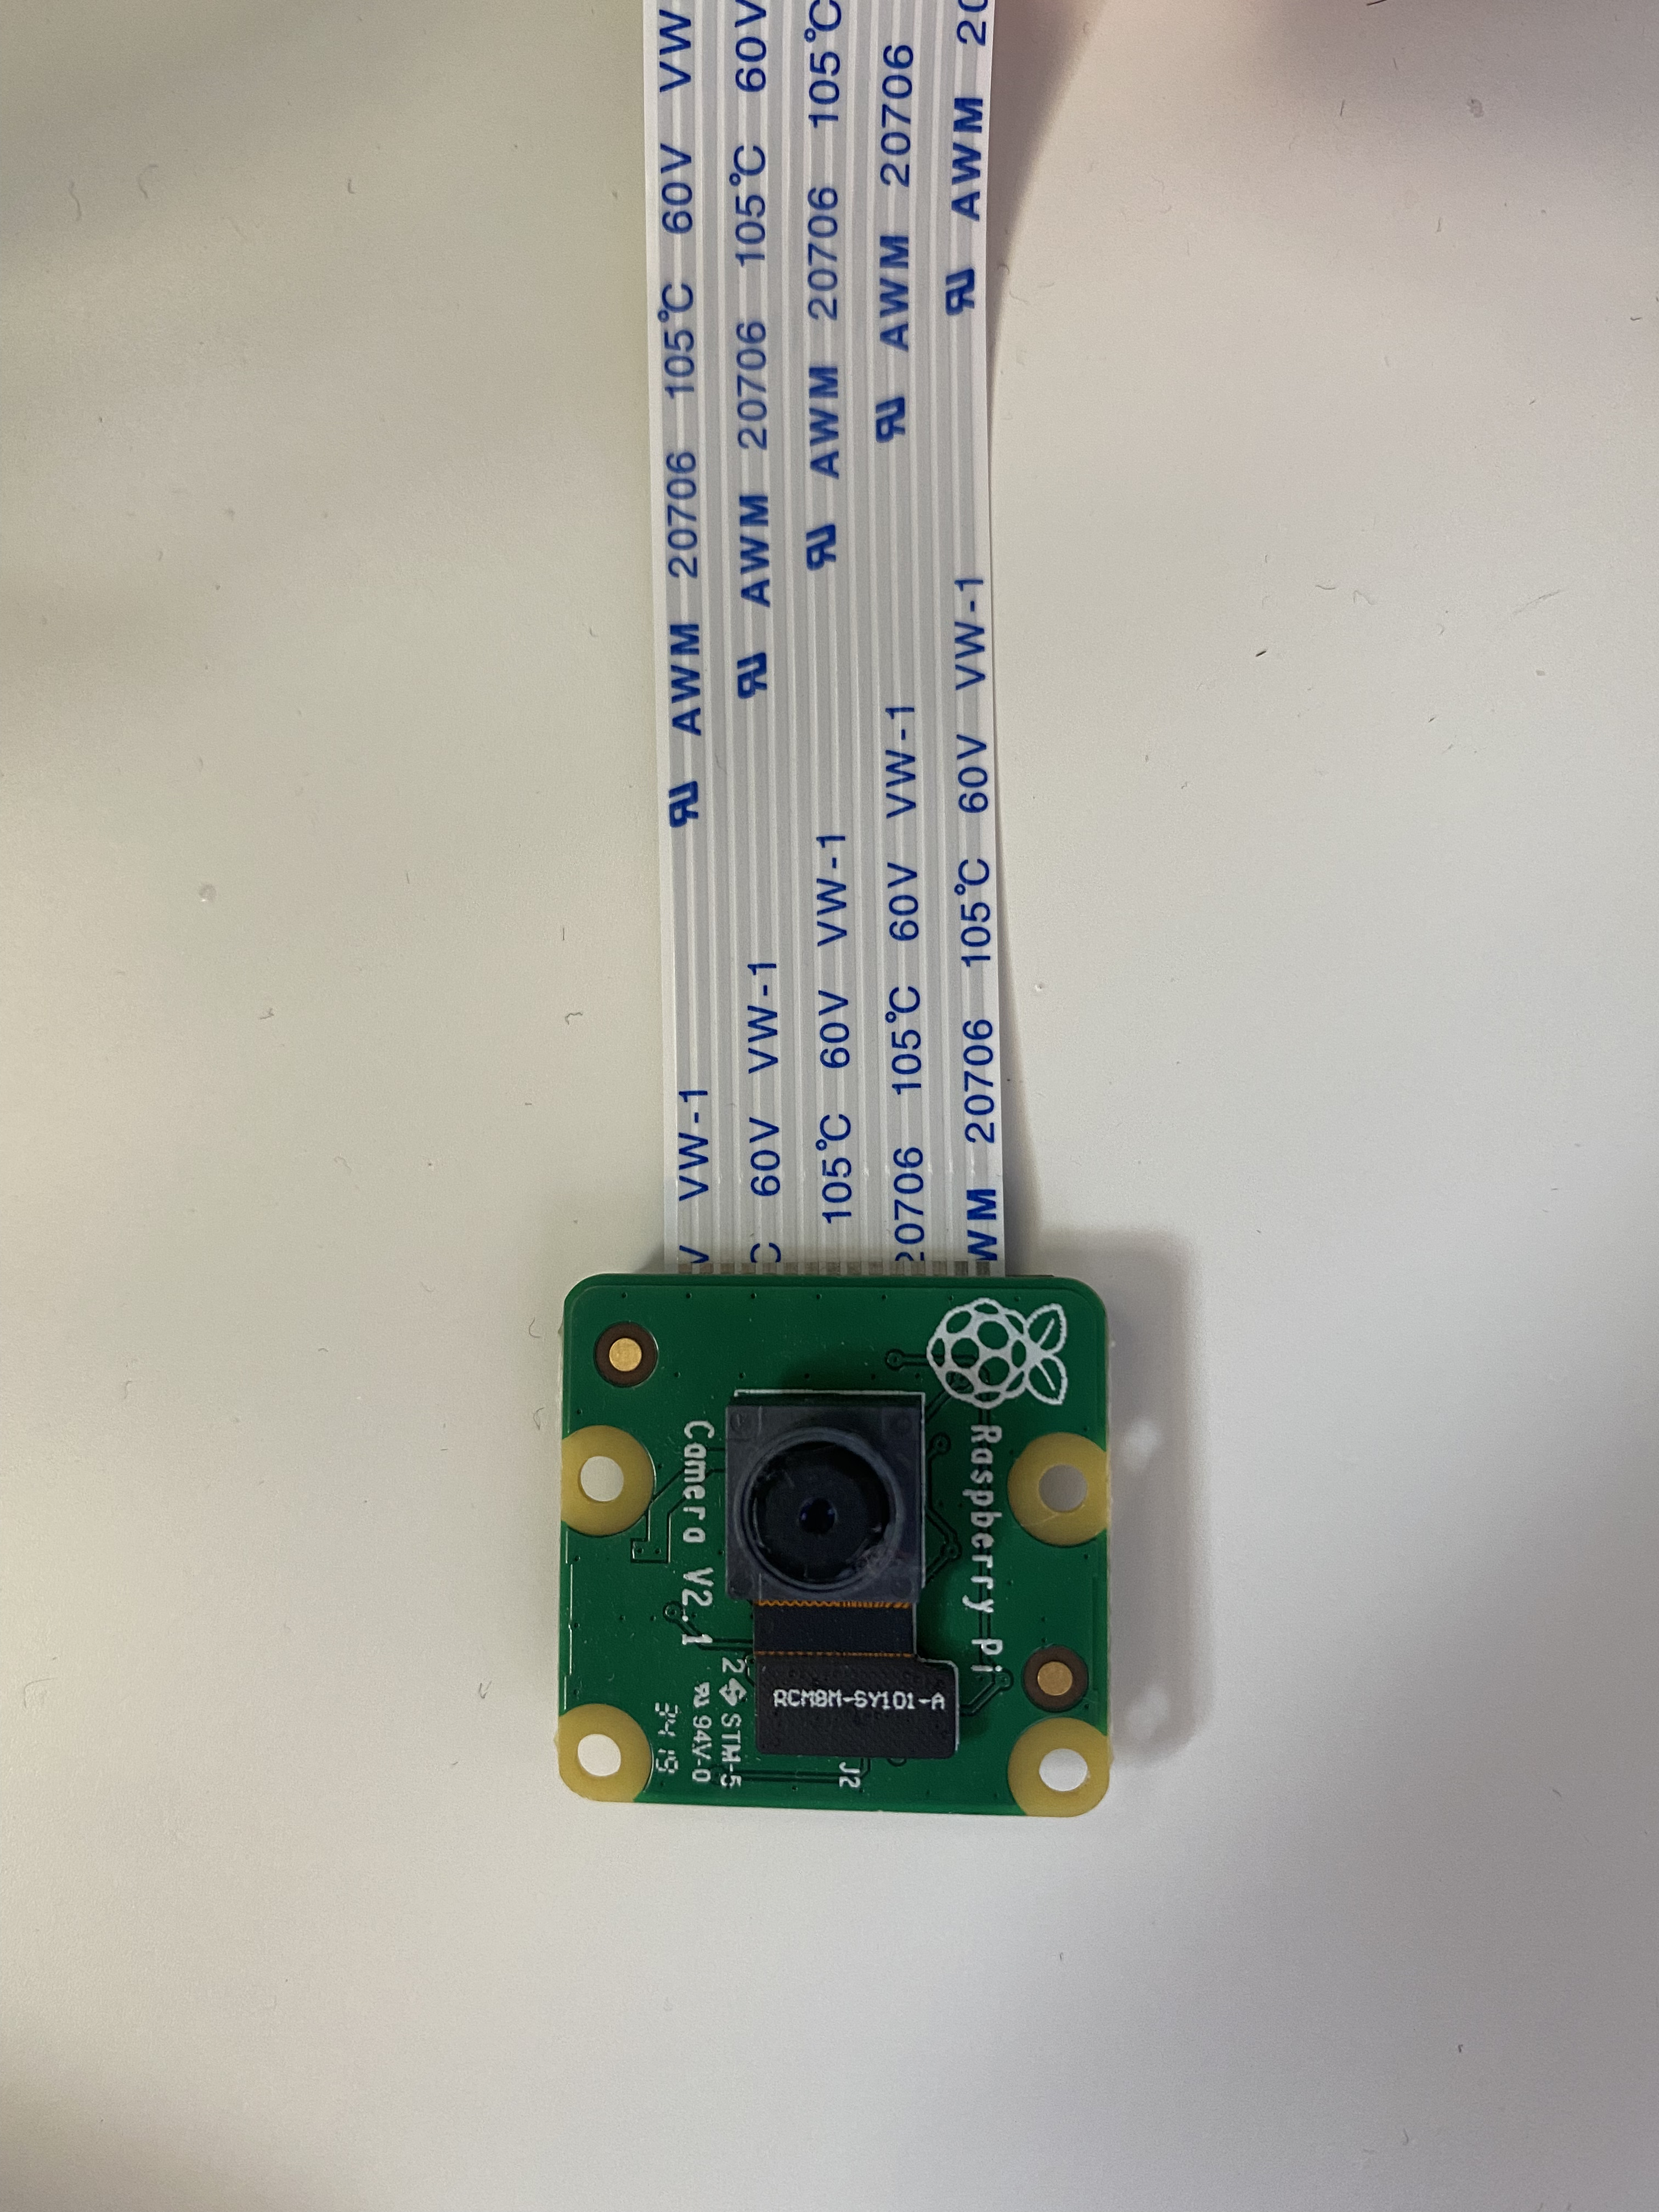
\includegraphics[width=6cm]{figs/picam}
  \end{center}
  \caption{Cámara de Raspberry.}
  \label{fig:picam}
\end{figure}\\
\end{itemize}

Además de los sensores, se han utilizado otros componentes como son resistencias, un led o un conversor analógico a digital para el correcto funcionamiento de los sensores y proporcionar mayor comprensión al funcionamiento del sistema.

En la figura \ref{fig:esquema} se puede ver un esquema de la conexión de los sensores mencionados en la Raspberry.
\begin{figure} [h!]
  \begin{center}
    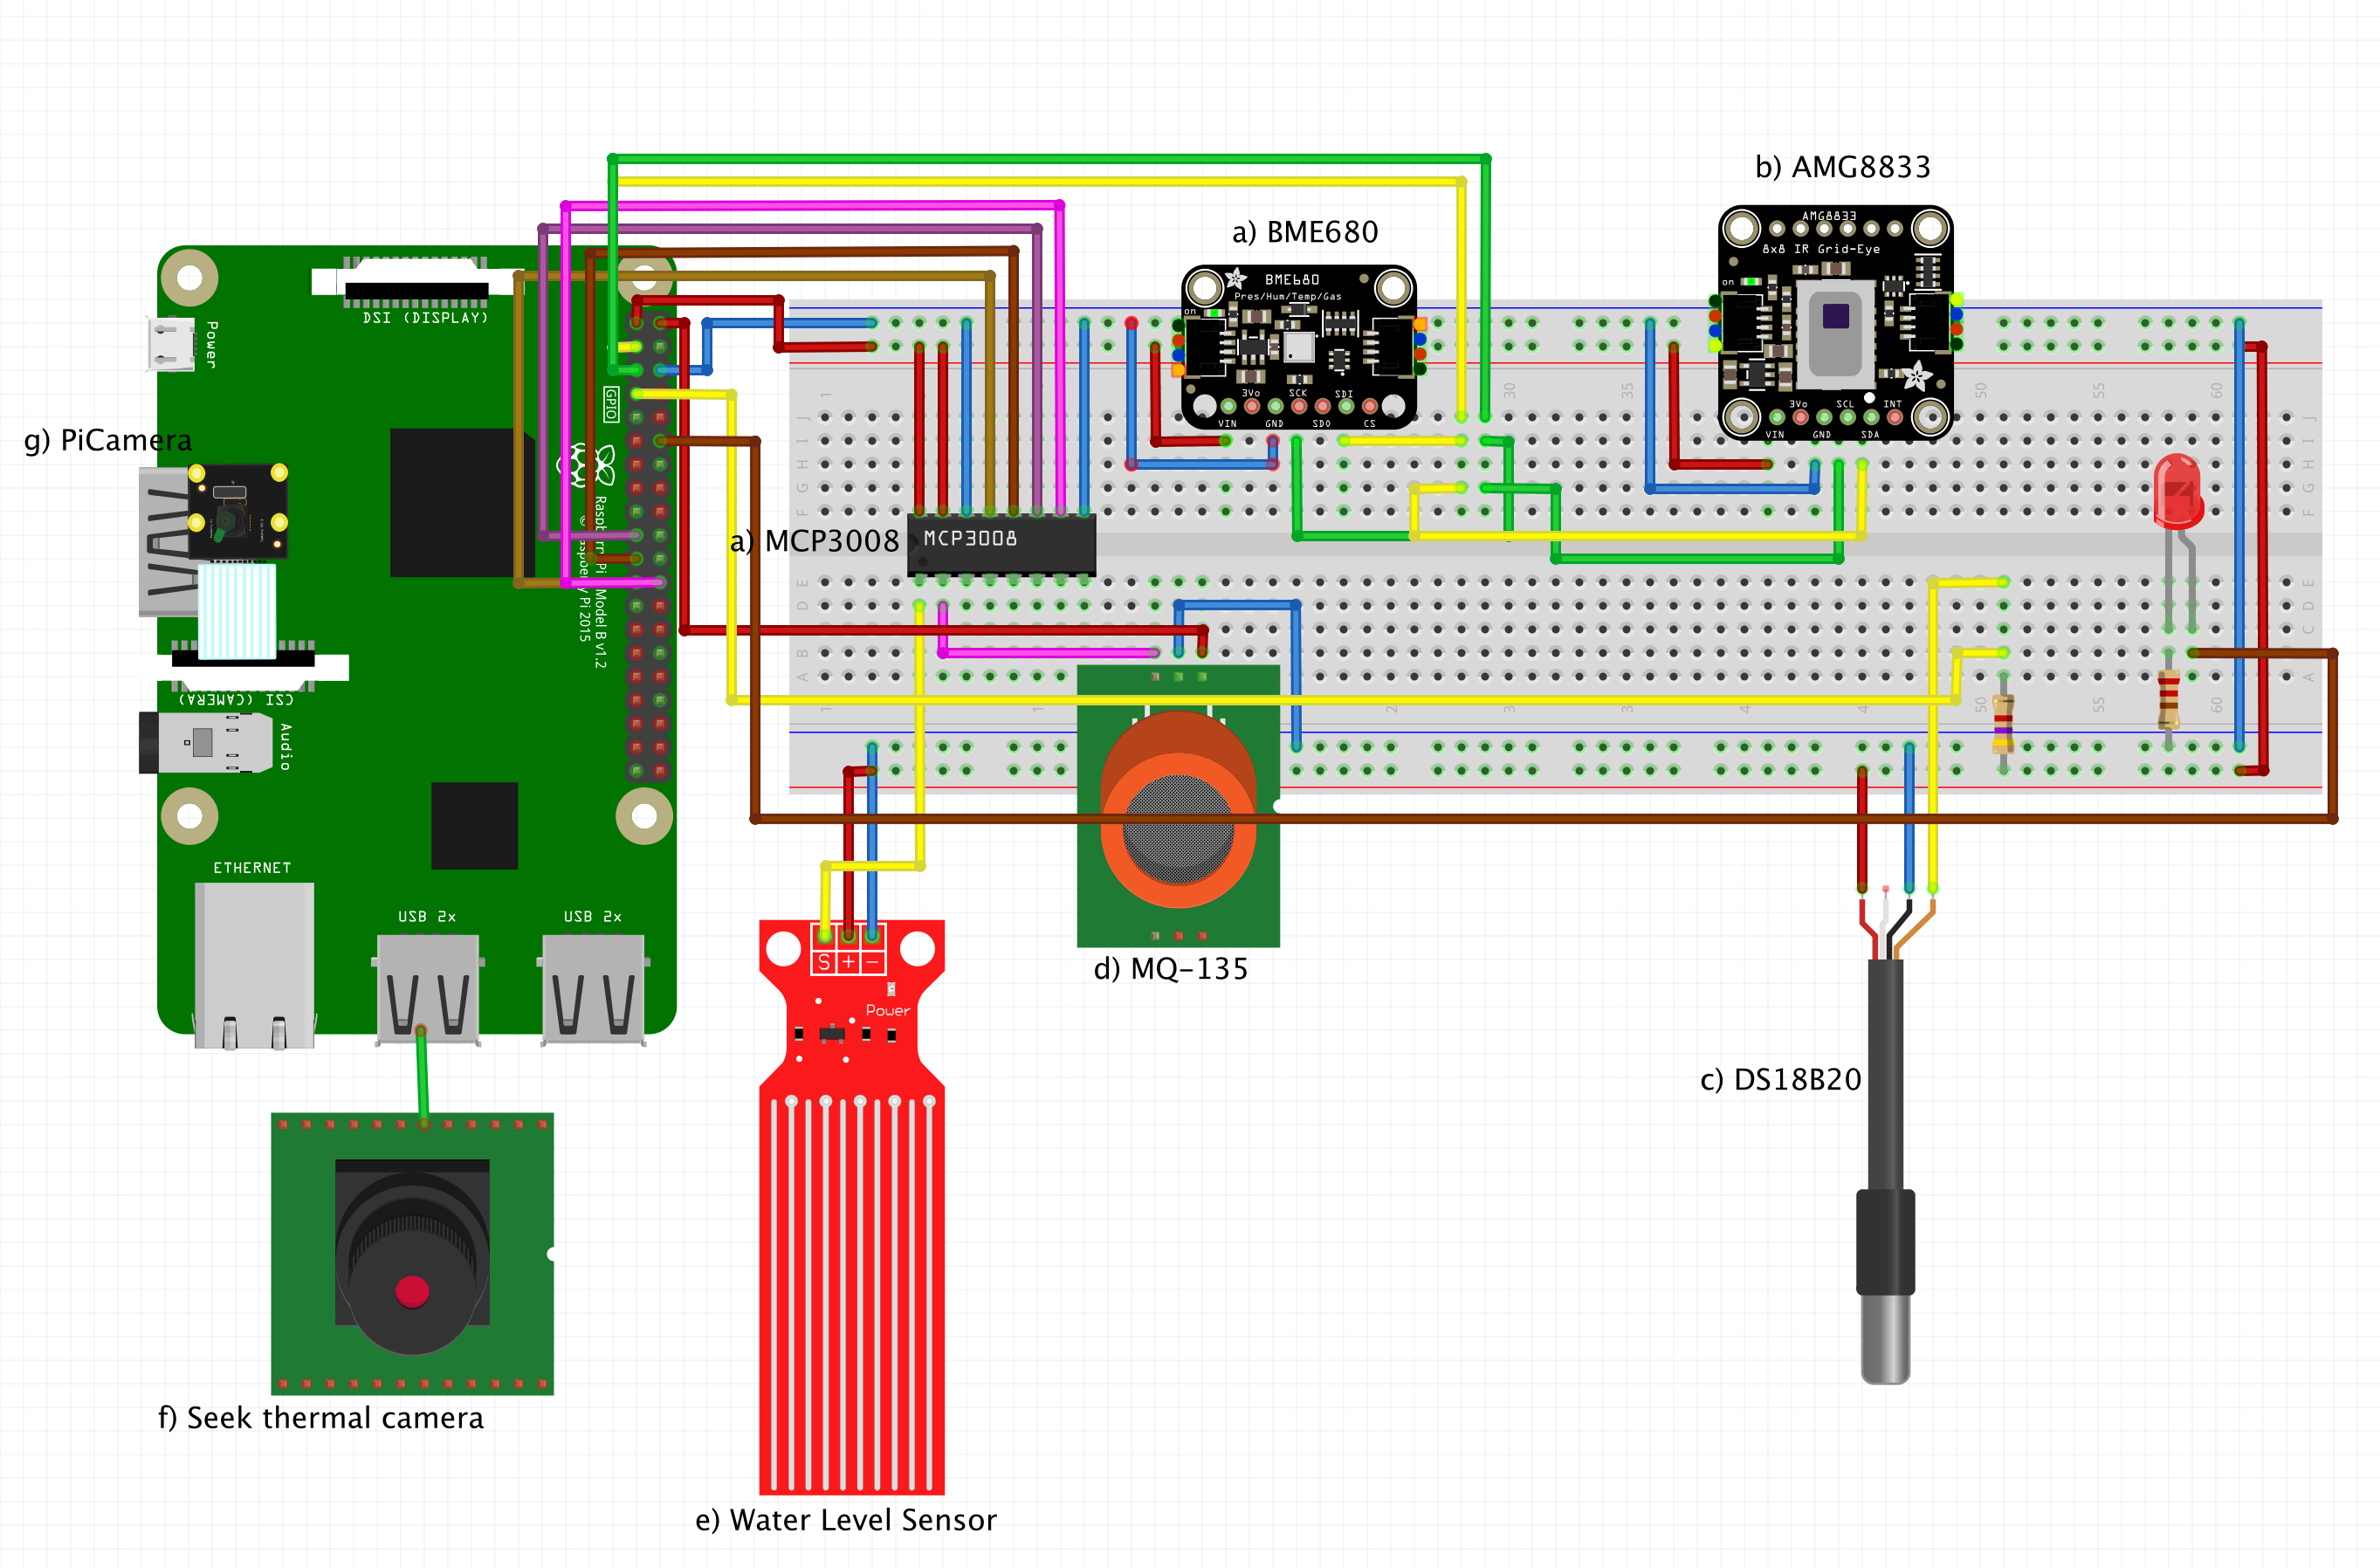
\includegraphics[width=14cm]{figs/esquema}
  \end{center}
  \caption{Esquema de conexiones.}
  \label{fig:esquema}
\end{figure}\\

\section{Software}
Tras disponer de la parte hardware, el equipo está preparado. Para que este equipo funcione, es necesario crear las instrucciones y reglas a través de programas o aplicaciones, esto es, la parte software.

En primer lugar ha sido necesaria la instalación de las librerías necesarias para el funcionamiento de todos los sensores. Después de la instalación, han surgido varios problemas al intentar leer de los distintos sensores. Uno de los problemas encontrado en dos sensores ---los que funcionabas con conexión i2c--- ha sido que la Raspberry no los detectaba.

Se pueden encontrar los errores que han surgido en la instalación y las respectivas soluciones para hacer funcionar todos los sensores en la wiki\footnote{\url{https://github.com/jmvega/tfg-icebollada/wiki/2.February-progress}} que se ha creado para realizar el proyecto.\\

\subsection{Fichero Python para lectura sensorial}
Durante este proceso, ha habido dos sensores que se han intentado utilizar sin éxito debido a que no tienen compatibilidad con Raspberry: CCS811, que mide la calidad del aire y AM2315, que mide la temperatura y humedad. Aun así, esto no ha sido un problema ya que son datos que se han podido obtener con otros sensores disponibles.\\

Se ha considerado que el usuario no tiene conocimiento para comprender los datos en crudo que ofrece un sensor, por tanto, ha sido necesario realizar diferentes cambios para ofrecer una comprensión fácil al usuario.

Se ha utilizado el programa Node-Red para ofrecer una interfaz al usuario, de forma que este sea capaz de ver la información del estado del sistema representada a través de widgets, que son pequeñas imágenes que proveen información visual. Así ha sido posible crear un interfaz ameno e intuitivo que el usuario puede comprender a través de algo más visual que valores numéricos.\\

Para poder mostrar todos los sensores en tiempo real en Node-Red, ha sido necesario disponer de un fichero de Python que  cada vez que se ejecute lea una sola vez de todos ellos. No debe leer continuamente ya que es la configuración de Node-Red la que se encarga de ello. En este fichero sólo se procesan los sensores que devuelven salidas numéricas, esto es, todos sensores excepto la PiCam \ref{fig:picam} y la cámara térmica \ref{fig:seek}. 

Para crear este fichero de una manera organizada, se ha creado una clase por cada sensor. El esquema de la clase de cada sensor se puede ver en la Figura \ref{fig:umlet}. 
\begin{figure} [h!]
  \begin{center}
    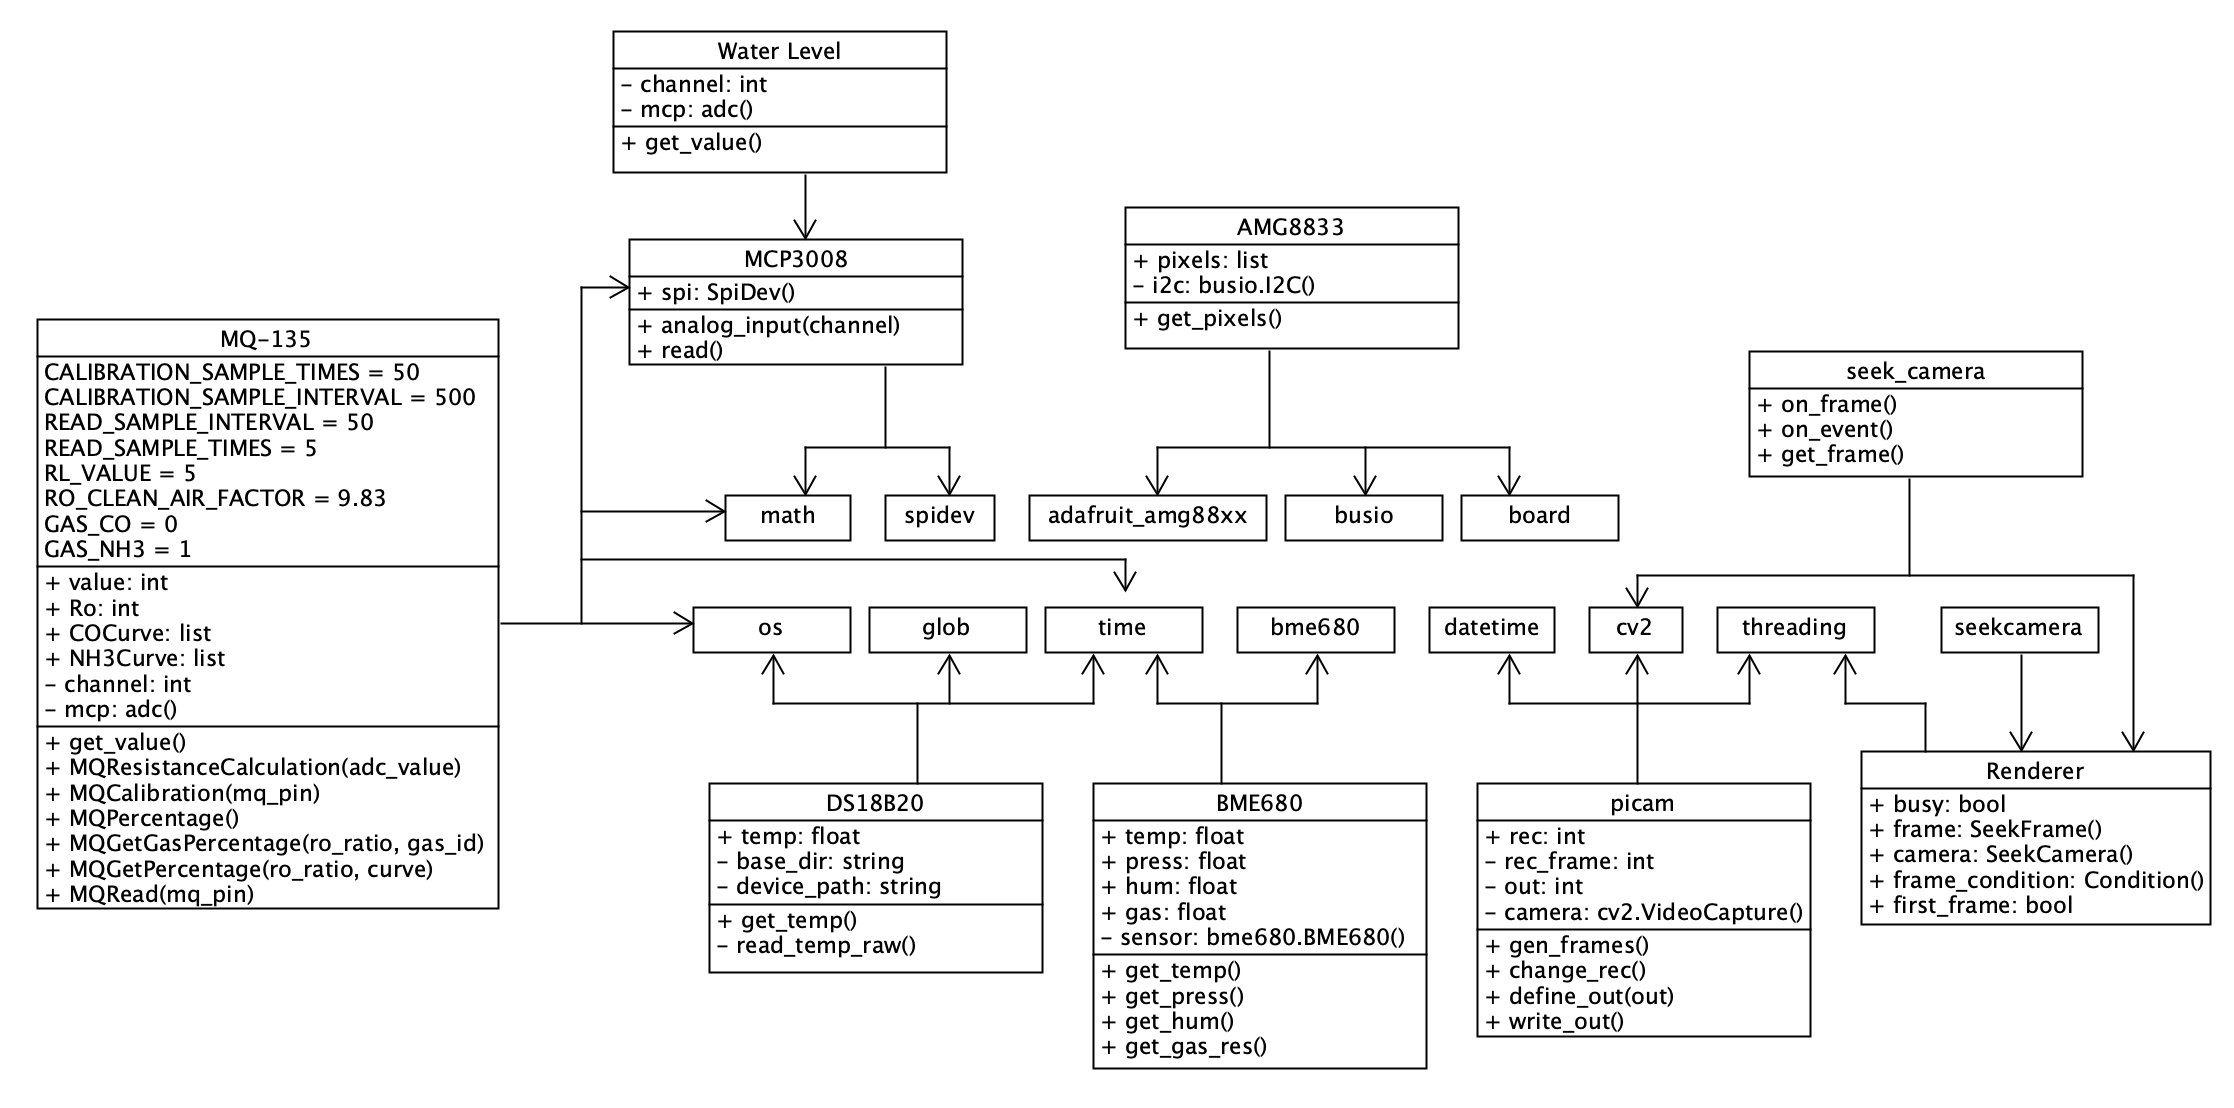
\includegraphics[width=16cm]{figs/umlet}
  \end{center}
  \caption{Esquema de clases de cada sensor.}
  \label{fig:umlet}
\end{figure}\\

Este fichero de Python utiliza la librería Threads para poder leer de manera concurrente todos los sensores, ahorrando tiempo y ganando eficacia. El código \ref{cod:threads} muestra cómo se crea un hilo ---o thread--- por cada sensor, siendo la lista del primer bucle una función que lee el valor del sensor respectivo.
\begin{code}[h]
\begin{lstlisting}[language=Python]
threads = []

for func in [x.ammo, x.bme, x.pix, x.lev, x.water_t]:
	threads.append(Thread(target=func))
	threads[-1].start()
	
for thread in threads:
	thread.join()
\end{lstlisting}
\caption[Función para crear un Thread por sensor y obtener su lectura]{Función para crear un Thread por sensor y obtener su lectura}
\label{cod:threads}
\end{code}

Además, este programa guarda las lecturas en un fichero csv por si fuese necesaria la comparación o estudio de datos a lo largo del tiempo. 

El fichero devuelve una cadena con la lectura de cada sensor, para poder procesar la salida en Node-Red.\\

\subsection{Creación de la interfaz de usuario}
Una vez creado este fichero, se ha procedido a crear la interfaz en Node-Red. Este programa funciona a través de diferentes tipos de nodos, que deben ser combinados para obtener el resultado deseado.

En primer lugar, a través del nodo de ejecución, representado en rojo con un engranaje, se pueden ejecutar ficheros que están en la máquina local. Este nodo es el que se ha utilizado para integrar en la aplicación el fichero que lee una vez todos los sensores.

Para obtener individualmente el valor de cada sensor, se ha utilizado otro nodo llamado nodo función, que permite incluir código directamente en Node-Red. Este nodo se ha utilizado para extraer de la salida del nodo ejecución el valor que le interesa.

Con estos dos nodos algunos sensores han estado listos para mostrar los valores en la interfaz de usuario (IU), por lo que solo ha sido necesario añadir el widget más adecuado para cada caso a través del nodo pertinente. Este ha sido el caso de los sensores MQ-135 \ref{fig:mq}, BME680 \ref{fig:bme} (en el caso de temperatura, presión y humedad) y DS18B20 \ref{fig:ds}.

En el caso de los otros sensores han sido necesarios otros cambios para obtener el resultado adecuado:
\begin{itemize}
	\item El sensor BME680 \ref{fig:bme} mide la resistencia del gas, pero se ha considerado que no es un parámetro intuitivo y no proporciona conocimiento al usuario. Por ello se ha utilizado otro nodo función que primero realiza la media de 50 lecturas de resistencia de gas y posteriormente establece la calidad del aire en función a la humedad y resistencia del aire.
	\item Durante diferentes pruebas, se ha detectado que el sensor que mide el nivel de agua \ref{fig:nivel} no es preciso a la hora de detectar la cantidad de agua presente, solamente es preciso detectando la presencia de esta.
	
	Por tanto, se ha optado por dividir en 4 rangos el nivel de agua, de tal manera que el usuario tenga una idea sobre la cantidad de agua presente. Aún así, el sensor no es suficientemente preciso a lo largo de diferentes pruebas y esta opción tampoco ha sido válida. 
	Como ajuste que dota de más precisión a este sensor, se ha incorporado un botón en la interfaz para poder calibrar el sensor cuando el recipiente esté lleno de agua. Todo el desarrollo y las pruebas que se han llevado a cabo con este sensor pueden ser encontradas en la wiki \footnote{\url{https://github.com/jmvega/tfg-icebollada/wiki/3.March-progress}} del proyecto.
	
	\item El sensor AMG8833 \ref{fig:amg} devuelve en su lectura una lista de 8x8 valores. Estos valores han sido convertidos a imagen ya que este sensor es una cámara térmica. Para este proceso ha sido necesario enlazar una serie de nodos hasta poder obtener la imagen más nítida, ya que la imagen obtenida originalmente ha sido una imagen de 8x8 píxeles que no alcanzaba a diferenciar objetos. De nuevo, tanto este progreso como las diferentes soluciones obtenidas se pueden encontrar en la wiki. 
\end{itemize}

Con estos ajustes realizados, se ha obtenido parte de la IU. Para hacerla más completa se ha incorporado un interruptor de forma que el usuario puede decidir si apagarla o bien mantenerla encendida, así como un nodo que regula la repetitividad del sistema cada 3 segundos.

La interfaz a este punto se puede ver en la imagen \ref{fig:ui_nocams}.
\begin{figure} [h!]
  \begin{center}
    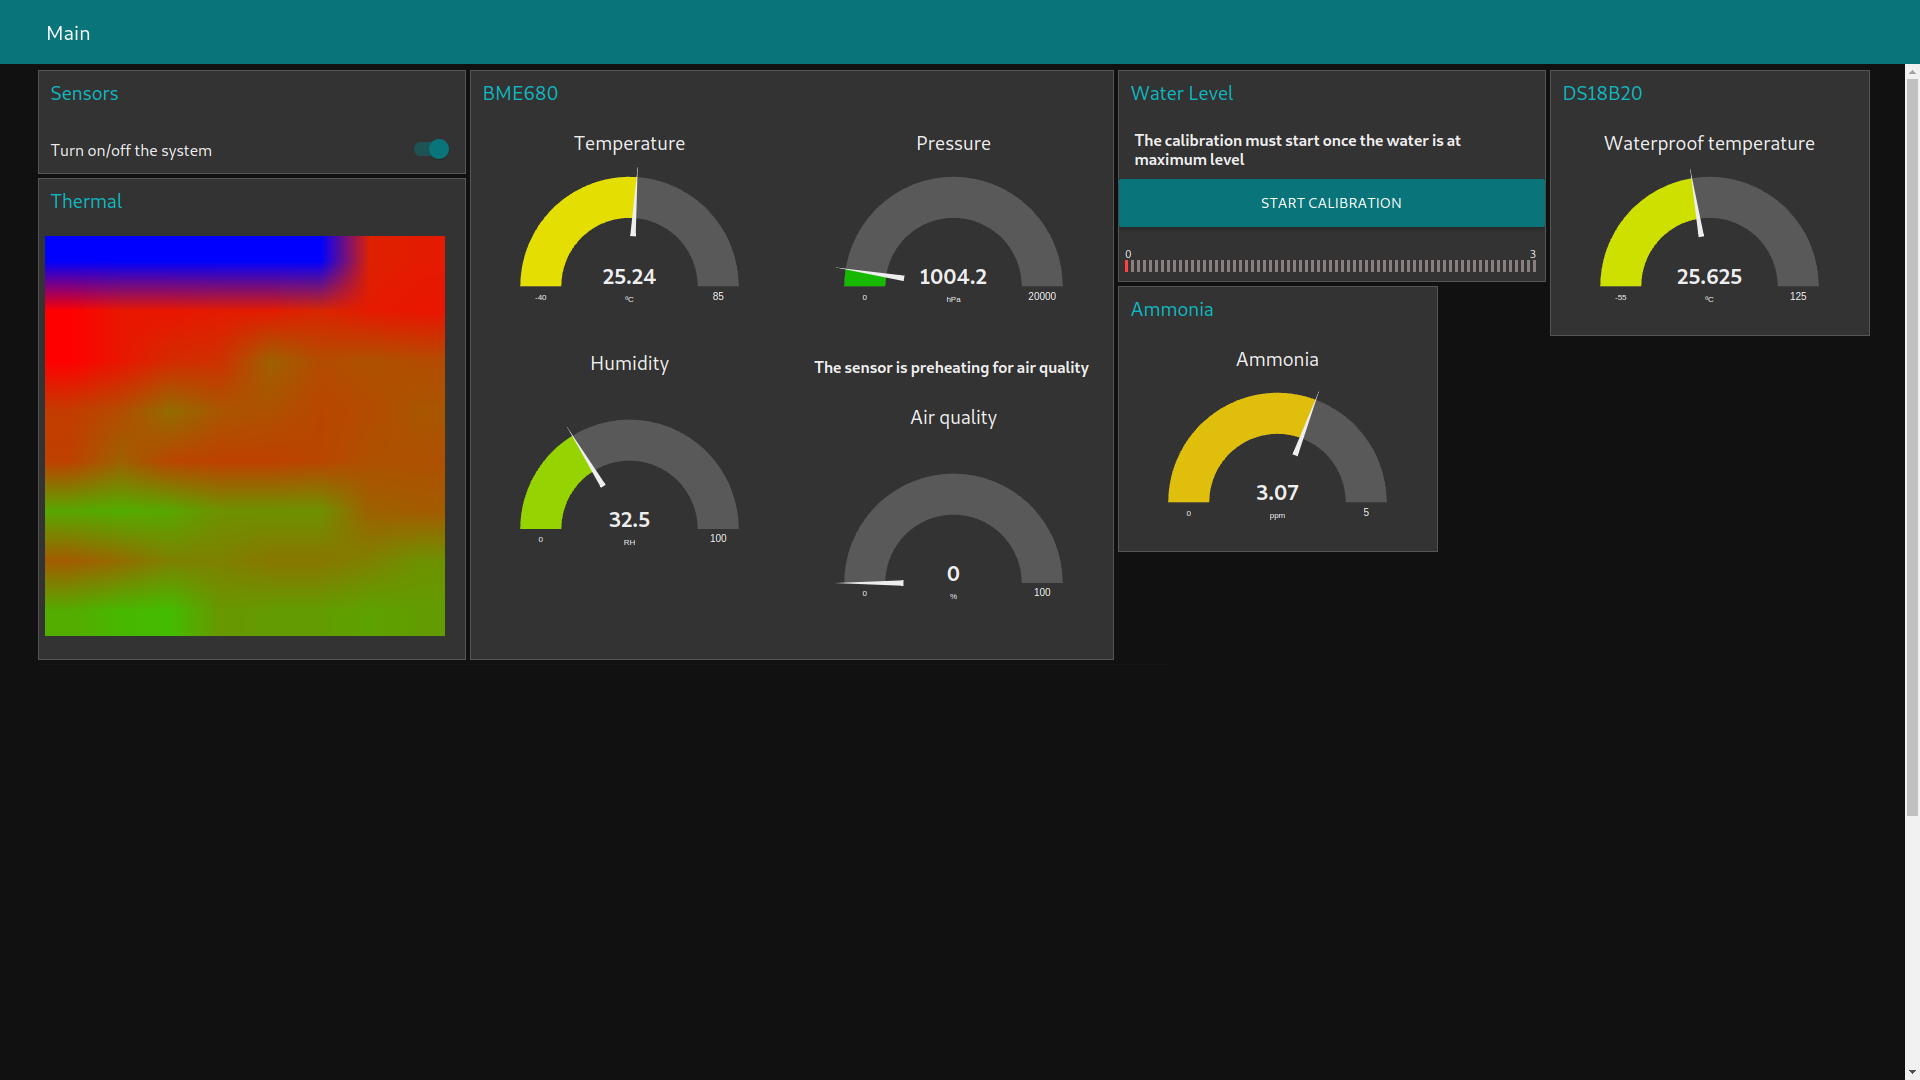
\includegraphics[width=16cm]{figs/ui_nocams}
  \end{center}
  \caption{IU sin los sensores cámaras.}
  \label{fig:ui_nocams}
\end{figure}\\

\subsection{Integración de las cámaras en la UI}
La creación de la interfaz en la subsección anterior no es completa, ya que faltan dos de los sensores que se utilizan en este trabajo: las cámaras.

Para poder visualizar las cámaras desde Node-Red debe ser a través del nodo template (que significa plantilla), que permite visualizar una dirección web. Por tanto ha sido necesario crear un servidor que permita visualizar las imágenes en un servidor y por tanto poder incluirlo en la IU. Para crear este servidor se ha utilizado Flask.\\

Se ha decidido crear una servidor por cada cámara. De esta manera se puede acceder solamente a una visualización o bien a las dos, según el interés del usuario. 

Para el funcionamiento de la cámara térmica Seek Thermal \ref{fig:seek} se ha utilizado la librería que tiene seek, que permite su visualización a través de OpenCV.

Para el funcionamiento de la PiCam \ref{fig:picam} se ha utilizado OpenCV tanto para su visualización como para la adición de la fecha y la hora en la visualización (Figura \ref{fig:fechayhora}). El código \ref{cod:fechayhora} muestra como se consigue.
\begin{figure} [h!]
  \begin{center}
    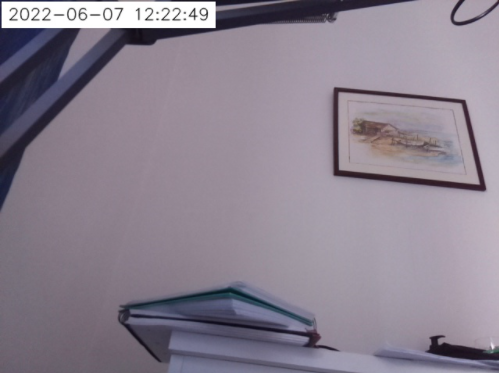
\includegraphics[width=8cm]{figs/fechayhora}
  \end{center}
  \caption{Incorporación de la fecha y hora en la visualización de la PiCam.}
  \label{fig:fechayhora}
\end{figure}\\

\begin{code}[h]
\begin{lstlisting}[language=Python]
ret, frame = self.__camera.read()
frame = cv2.rectangle(frame, (2,2), (275,35), (255,255,255), -1)
frame = cv2.putText(frame, str(datetime.datetime.now().replace(microsecond=0)), (10,25), cv2.FONT_HERSEY_SIMPLEX, 0.7, (0,0,0), 1, cv2.LINE_AA))
\end{lstlisting}
\caption[Código para crear un rectángulo y escribir la fecha actual sobre el.]{Código para crear un rectángulo y escribir la fecha actual sobre el.}
\label{cod:fechayhora}
\end{code}

\section{Verbatim}

Para mencionar identificadores usados en el código ---como nombres de funciones o variables--- en el texto, usa el entorno literal o verbatim \verb|hypothesizeParallelograms()|. También se puede usar este entorno para varias líneas, como se ve a continuación:

\begin{verbatim}
void Memory::hypothesizeParallelograms () {
  // add your code here
}
\end{verbatim}

\section{Ecuaciones}

Si necesitas insertar alguna ecuación, puedes hacerlo. Al igual que las figuras, no te olvides de referenciarlas. A continuación se exponen algunas ecuaciones de ejemplo: Ecuación \ref{ec:ec1} y Ecuación \ref{ec:ec2}.

\begin{myequation}[h]
\begin{equation}
H = 1 - \frac{\sum_{i=0}^{N}\frac{(\frac{d_{j_s} + d_{j_e}}{2})}{N}}{M}
\nonumber
\label{ec:ec1}
\end{equation}
\caption[Ejemplo de ecuación con fracciones]{Ejemplo de ecuación con fracciones}
\end{myequation} 

\begin{myequation}[h]
\begin{equation}
v(entrada)= \left\{
	\begin{array}{lcc}
		0 & \mbox{if} & \epsilon_t < 0.1\\
		K_p\cdot{(T_{t}-T)} & \mbox{if}& 0.1 \leq \epsilon_t < M_t\\
		K_p \cdot M_t & \mbox{if}& M_t < \epsilon_t
	\end{array}
\right.
\label{ec:ec2}
\end{equation}
\caption[Ejemplo de ecuación con array y letras y símbolos especiales]{Ejemplo de ecuación con array y letras y símbolos especiales}
\end{myequation}

\section{Tablas o cuadros}

Si necesitas insertar una tabla, hazlo dígnamente usando las propias tablas de \LaTeX, no usando pantallazos e insertándolas como figuras... En el Cuadro \ref{cuadro:ejemplo} vemos un ejemplo.

\begin{table}[H]
\begin{center}
\begin{tabular}{|c|c|}
\hline
\textbf{Parámetros} & \textbf{Valores} \\
\hline
Tipo de sensor & Sony IMX219PQ[7] CMOS 8-Mpx \\
Tamaño del sensor & 3.674 x 2.760 mm (1/4" format) \\
Número de pixels & 3280 x 2464 (active pixels) \\
Tamaño de pixel & 1.12 x 1.12 um \\
Lente & f=3.04 mm, f/2.0 \\
Ángulo de visión & 62.2 x 48.8 degrees \\
Lente SLR equivalente & 29 mm \\
\hline
\end{tabular}
\caption{Parámetros intrínsecos de la cámara}
\label{cuadro:ejemplo}
\end{center}
\end{table}

